\input{../../common/slide-common-header.tex}

\newcommand{\orgNum}{0}
\newcommand{\orgTopic}{org meeting}
\newcommand{\orgKey}{syllabus, contacts}

\newcommand{\introNum}{1}
\newcommand{\introTopic}{introduction to multithreading}
\newcommand{\introKey}{concurrency, parallelism, agents, threads, scheduler, Amdahl's law, race condition, deadlock, wait-for graph}

\newcommand{\basicNum}{2}
\newcommand{\basicTopic}{basic concepts}
\newcommand{\basicKey}{mutex, acquisition order, reentrancy, fairness, data locking, code locking, signalling, condition variable, lost signal, spurious wakeup}

\newcommand{\syncPrimitivesNum}{3}
\newcommand{\syncPrimitivesTopic}{advanced synchronization primitives}
\newcommand{\syncPrimitivesKey}{monitor, latch, barrier, thundering herd, semaphore, read-write lock, thread pool, executor, producer-consumer, fork-join, load balancing}

\newcommand{\patternsNum}{4}
\newcommand{\patternsTopic}{advanced synchronization concepts}
\newcommand{\patternsKey}{interruption, cancellation, partitioning, privatization, replication, thread-local, ownership}

\newcommand{\extraBasicsNum}{5}
\newcommand{\extraBasicsTopic}{additional topics of practical concurrency}
\newcommand{\extraBasicsKey}{documenting protocols and classes, checking concurrent invariants, stress testing, execution trace analysis, estimating required testing effort, static and dynamic checks, scheduling randomization, model checking}

\newcommand{\foundationsNum}{6}
\newcommand{\foundationsTopic}{theoretical foundations of concurrency}
\newcommand{\foundationsKey}{timeline, events, precedence, 2-thread mutual exclusion, deadlock freedom, starvation freedom, N-thread mutual exclusion, sequential objects and specifications, concurrent objects, linearizability}

\newcommand{\foundationsPlusNum}{7}
\newcommand{\foundationsPlusTopic}{progress guarantees, concurrent operations hierarchy, consensus number}
\newcommand{\foundationsPlusKey}{obstruction-free, lock-free, wait-free, safe register, regular register, atomic register, register snapshot, consensus number}

\newcommand{\atomicsNum}{8}
\newcommand{\atomicsTopic}{introduction to atomics}
\newcommand{\atomicsKey}{read-modify-write, get-and-add, compare-and-swap, spin lock, lock-free stack, ABA problem}

% TODO: taxonomy of queues, 

\newcommand{\cacheCoherencyNum}{9}
\newcommand{\cacheCoherencyTopic}{cache coherency}
\newcommand{\cacheCoherencyKey}{cache memory hierarchy, cache coherency protocol, store-buffer, load-buffer, invalidate-queue, memory barrier, hardware memory model, weak memory model, litmus tests}

\newcommand{\langMMNum}{10}
\newcommand{\langMMTopic}{language memory model}
\newcommand{\langMMKey}{compiler optimizations, compiler barriers, language memory model, strict consistency, threads cannot be implemented as a library, visibility, volatile}

\newcommand{\advancedConcurrencyNum}{11}
\newcommand{\advancedConcurrencyTopic}{advanced locking}
\newcommand{\advancedConcurrencyKey}{Anderson Queue Lock, CLH, MCS, check-then-act, spin-then-park}

% TODO: work distribution, work stealing, taxonomy of parallel problems, single LIFO cell optimization, RAT

\newcommand{\userSpaceThreadingNum}{12}
\newcommand{\userSpaceThreadingTopic}{user-space threading}
\newcommand{\userSpaceThreadingKey}{berkley socket, blocking and non-blocking IO, callback-hell, async-await, continuation-passing-style, fibers/coroutines/green threads, stackful vs stackless}


\newcommand{\designNum}{13}
\newcommand{\designTopic}{designing concurrent systems}
\newcommand{\designKey}{park/unpark, synchronizer, futex/wait-on-address, plan9 approach, race-finders, ForkJoinPool/CoroutineCarriers/UIthread, observability, structured concurrency}

\newcommand{\frameworksAndDistributedNum}{14}
\newcommand{\frameworksAndDistributedTopic}{multi-agent systems}
\newcommand{\frameworksAndDistributedKey}{auto-parallelization languages and frameworks, semi-automatic synchronization, distributed systems, consensus protocols}



\title[]{Lecture \concurrentQueuesNum: \concurrentQueuesNumTopic}
\subtitle[]{\concurrentQueuesNumKey}
\author[]{Alexander Filatov\\ filatovaur@gmail.com}

\date{}

\begin{document}

\begin{frame}
  \titlepage
  \url{https://github.com/Svazars/parallel-programming/blob/main/slides/pdf/l13.pdf}
\end{frame}

\begin{frame}{In previous episodes}

Threading models\footnote{\tiny\url{https://en.wikipedia.org/wiki/Thread_(computing)#Threading_models}}
\begin{itemize}
  \item 1:1 threading (user thread = OS thread, \texttt{ThreadFactory})
  \item N:1 threading (event loop, \texttt{newSingleThreadExecutor})
  \item N:M threading (coroutines, \texttt{newFixedThreadPool})
  \item Lazy/on-demand thread creation (\texttt{newCachedThreadPool})
\end{itemize}

Heavyweight OS threads affect programming style 
\begin{itemize}
  \item Task pools vs long-running tasks
  \item Task pools vs blocking methods
  \item Asynchronous I/O and callback-based programming
\end{itemize}

User-space scheduling:
\begin{itemize}
  \item Stackless coroutines (CPS and suspend/resume coloring)
  \item Stackful coroutines (low-level: scheduling policy, context switch, preemption)
\end{itemize}

\end{frame}

\begin{frame}{Lecture plan}
\tableofcontents
\end{frame}

\section{Queues for mutual exclusion}
\showTOC

\questiontime{Name queue-based mutexes that you already know}

\begin{frame}[t,fragile]{Queue-based mutexes}

\begin{itemize}
  \item<2-> Array-based: Anderson lock
  \item<4-> LinkedList-based: CLH lock
  \item<6-> LinkedList-based: MCS lock
\end{itemize}

\begin{tabular}{lll}
\only<3->{ \begin{center} 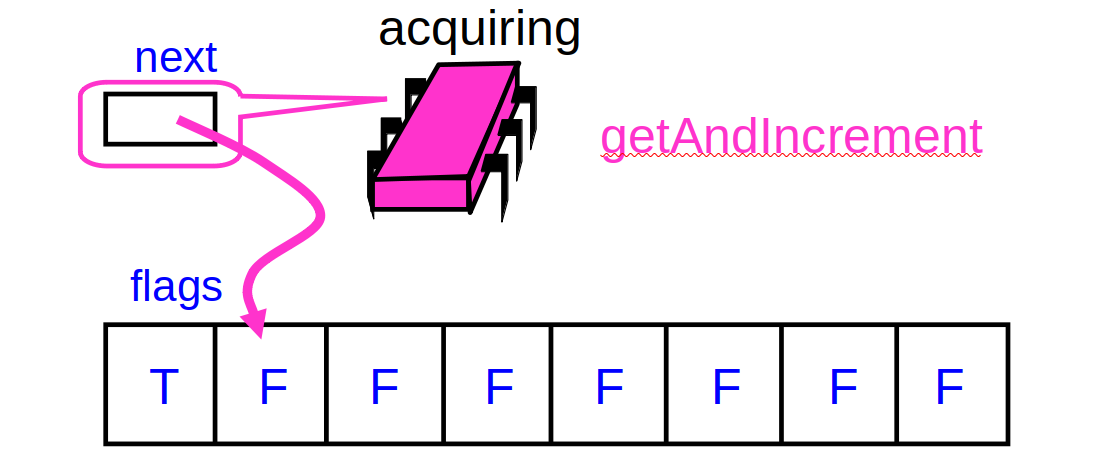
\includegraphics[width=0.3\textwidth]{./pics/alock-list.png} \end{center} }
&
\only<5->{ \begin{center} 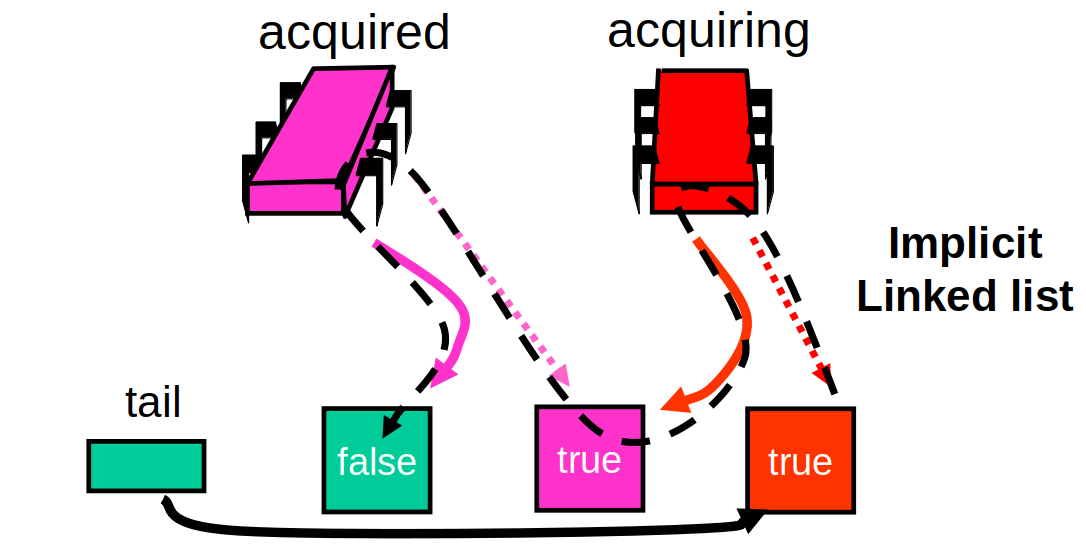
\includegraphics[width=0.3\textwidth]{./pics/clh-list.png} \end{center} }
&
\only<7->{ \begin{center} 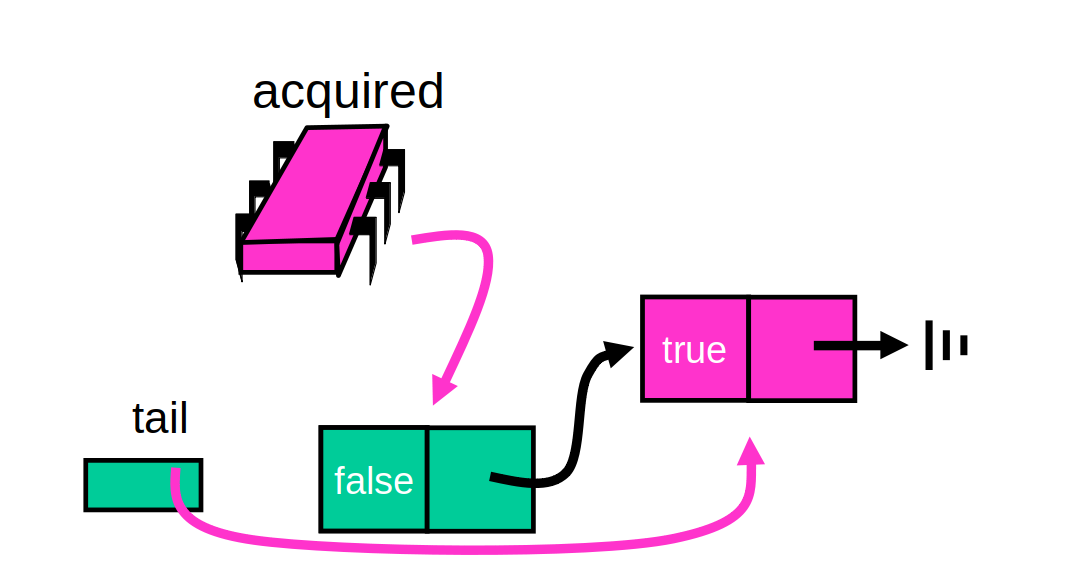
\includegraphics[width=0.3\textwidth]{./pics/mcs-post.png} \end{center} }
\end{tabular}

\only<8->{
\textbf{Idea}: select container (LIFO, FIFO, priority queue) and use it to 
\begin{itemize}
 \item register competitors
 \item maintain admission policy
\end{itemize}  
}
\end{frame}


\begin{frame}[fragile]{FIFO queue for mutual exclusion}

\begin{minted}{java}
class FIFOLock implements Lock {
  private Queue q = ...
  void lock() {
    myNode = new Node();
    q.enqueue(myNode);
    while (true) { if (q.peek() == myNode) return; /* it is my turn */ }            
  }
  void unlock() {
    prevHead = q.dequeue(); // let other thread go
    assert prevHead == myNode; // could I delete myNode right now?
  }}
\end{minted}

\pause

Could be extended with spin-then-park and cancellation\footnote<2->{\tiny\url{https://docs.oracle.com/en/java/javase/11/docs/api/java.base/java/util/concurrent/locks/LockSupport.html}}

\end{frame}

\questiontime{How to implement mutex using lock-free LIFO stack?}

\begin{frame}[fragile]{Queues and mutexes: summary}

Thread-safe FIFO container could be transformed into mutex
\begin{itemize}
  \item admission policy control "out of the box"
  \item easy to associate data with every entering thread (e.g. thread-local memory for spinning)
  \item must maintain high level of concurrent consistency
  \begin{itemize}
      \item Strong FIFO
      \item Multiple enqueuers, Single dequeuer
  \end{itemize}  
\end{itemize}
\end{frame}

\questiontime{Name other usage scenarios for concurrent queues}

\section{Design space}
\showTOC

\begin{frame}[fragile]{Queues: where to use}

\begin{itemize}
  \item Concurrency control
  \begin{itemize}
    \pause \item \texttt{Lock} (\texttt{lock} $\approx$ \texttt{enqueue}, \texttt{unlock} $\approx$ \texttt{dequeue})
    \pause \item \texttt{ConditionVariable} (\texttt{signal} $\approx$ \texttt{enqueue}, \texttt{await} $\approx$ \texttt{dequeue})
    \pause \item \texttt{CountDownLatch} (\texttt{countDown} $\approx$ \texttt{dequeue}, \texttt{await} $\approx$ \texttt{isEmpty})
    \pause \item \texttt{Semaphore} (\texttt{acquire} $\approx$ \texttt{dequeue}, \texttt{release} $\approx$ \texttt{enqueue})
    \pause \item PoisonPill/ShutdownSignal pattern\footnote<6->{\tiny\url{https://java-design-patterns.com/patterns/poison-pill/#benefits-and-trade-offs-of-poison-pill-pattern}}
    \pause \item ...
  \end{itemize}

  \pause
  \item Data transfer
  \begin{itemize}
    \pause \item Push-based producer-consumer
    \pause \item Backpressure/reactive publisher-subscriber
  \end{itemize}  
  
  \pause
  \item Load balancing
  \begin{itemize}
    \pause \item Work arbitrage, work dealing, work stealing
  \end{itemize}  
\end{itemize}

\pause
What \textit{precisely} do we need from thread-safe container?

\end{frame}

\begin{frame}[t,fragile]{Queues: design space}

\begin{itemize}
  \pause \item Ordering guarantees
  \begin{itemize}
    \pause \item Strong FIFO \pause (linearizable to sequential queue)
    \pause \item Per-producer FIFO \pause (items enqueued by $i$-th producer are dequeued in FIFO order)
    \pause \item Best-effort FIFO
    \pause \item No ordering guarantees 
  \end{itemize}
\end{itemize}
\end{frame}

\begin{frame}[t,fragile,noframenumbering]{Queues: design space}

\begin{itemize}
  \item Ordering guarantees
  \begin{itemize}
    \item Strong FIFO, Per-producer FIFO, Best-effort FIFO, Nothing    
  \end{itemize}
  \pause \item Delivery guarantees 
  \begin{itemize}
    \pause \item Immediate vs Delayed (e.g. buffering) vs Eventual (e.g. dynamic routing) 
    \pause \item Guaranteed vs Possible loss (e.g. UDP)
    \pause \item Unique vs Possible duplicate 
    \begin{itemize}
      \pause \item Same item visible to competing dequeuers
      \pause \item Message resent under some condition
    \end{itemize}
  \end{itemize}
\end{itemize}
\end{frame}

\begin{frame}[t,fragile,noframenumbering]{Queues: design space}

\begin{itemize}
  \item Ordering guarantees
  \begin{itemize}
    \item Strong FIFO, Per-producer FIFO, Best-effort FIFO, Nothing    
  \end{itemize}
  \item Delivery guarantees 
  \begin{itemize}
    \item Immediate, Delayed, Eventual, Guaranteed, Unique
  \end{itemize}
  \pause \item Supported concurrency
  \begin{itemize}
    \pause \item Single Producer Single Consumer (SPSC)
    \pause \item Multiple Producers Single Consumer (MPSC)
    \pause \item Single Producer Multiple Consumers (SPMC)
    \pause \item Multiple Producers Multiple Consumers (MPMC)    
  \end{itemize}
\end{itemize}
\end{frame}

\begin{frame}[t,fragile,noframenumbering]{Queues: design space}

\begin{itemize}
  \item Ordering guarantees
  \begin{itemize}
    \item Strong FIFO, Per-producer FIFO, Best-effort FIFO, Nothing    
  \end{itemize}
  \item Delivery guarantees 
  \begin{itemize}
    \item Immediate, Delayed, Eventual, Guaranteed, Unique
  \end{itemize}
  \item Supported concurrency
  \begin{itemize}
    \item SPSC, MPSC, SPMC, MPMC    
  \end{itemize}

  \pause \item Capacity
  \begin{itemize}
    \pause \item Bounded, Unbounded
  \end{itemize}

  \pause \item API behaviour
  \begin{itemize}
    \pause \item \textit{total} methods do not wait (\texttt{dequeue} throws \texttt{EmptyException})
    \pause \item \textit{partial} methods may wait for condition (\texttt{enqueue} awaits empty slot in bounded queue)
    \pause \item \textit{synchronous} methods wait for overlapping method (\texttt{enqueue} awaits paired \texttt{dequeue})    
  \end{itemize}
\end{itemize}

\pause

We will look at some points in this design space

\end{frame}


\section{Unbounded lock-free queue}
\showTOC

\begin{frame}{Unbounded MPMC linearizable total queue}
\begin{itemize}
    \item Strong FIFO    
    \item MPMC
    \item Unbounded
    \item Total
    \pause
    \item Lock-free
\end{itemize}
\end{frame}


\begin{frame}[fragile]{Lock-Free Queue}
\only<1>{ \begin{center} 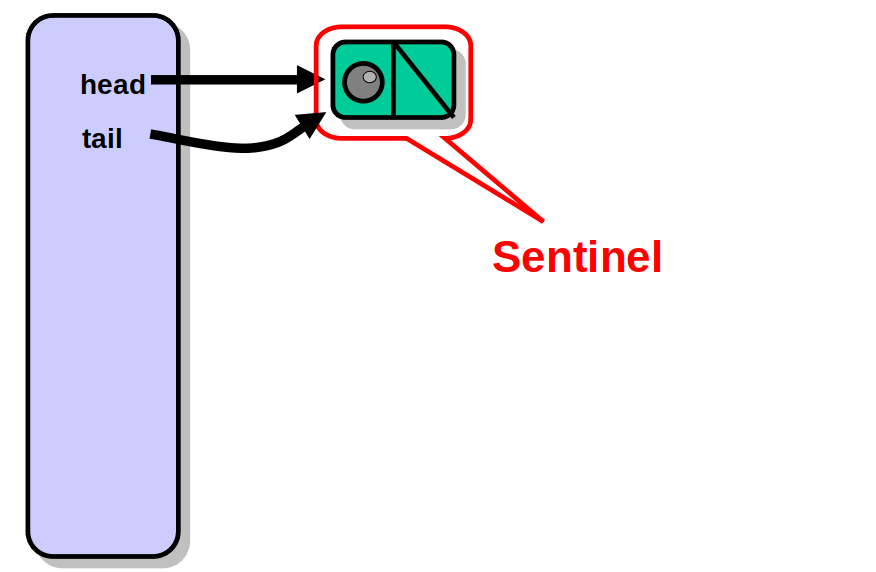
\includegraphics[width=0.7\textwidth]{./pics/unbound-mpmc/90.png} \end{center} }
\end{frame}

\begin{frame}[fragile]{Enqueue}
\only<1>{ \begin{center} 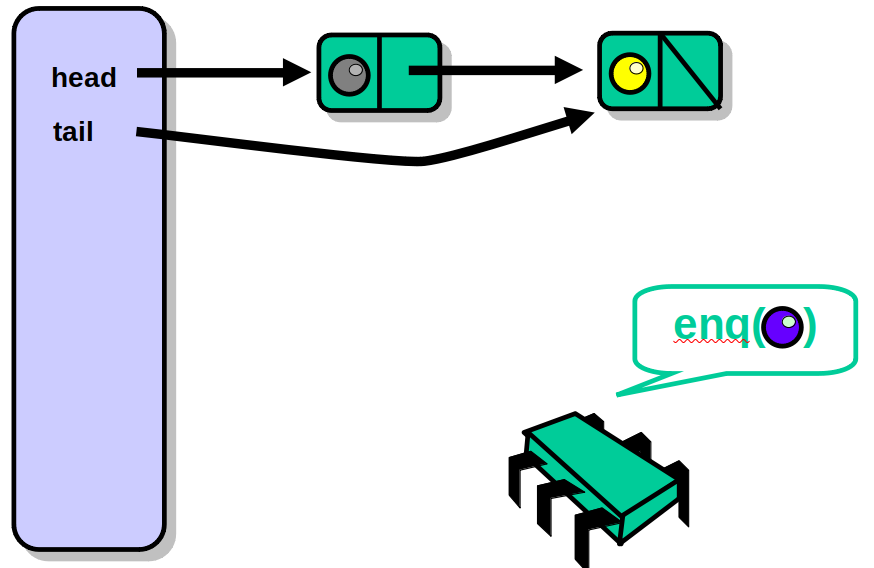
\includegraphics[width=0.7\textwidth]{./pics/unbound-mpmc/92.png} \end{center} }
\only<2>{ \begin{center} 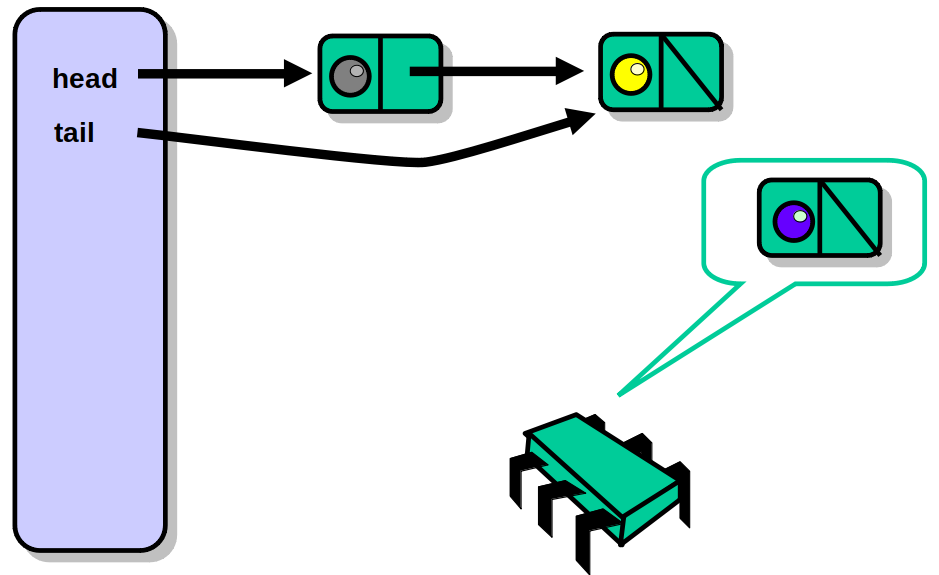
\includegraphics[width=0.7\textwidth]{./pics/unbound-mpmc/93.png} \end{center} }
\end{frame}

\begin{frame}[fragile]{Logical enqueue}
\only<1>{ \begin{center} 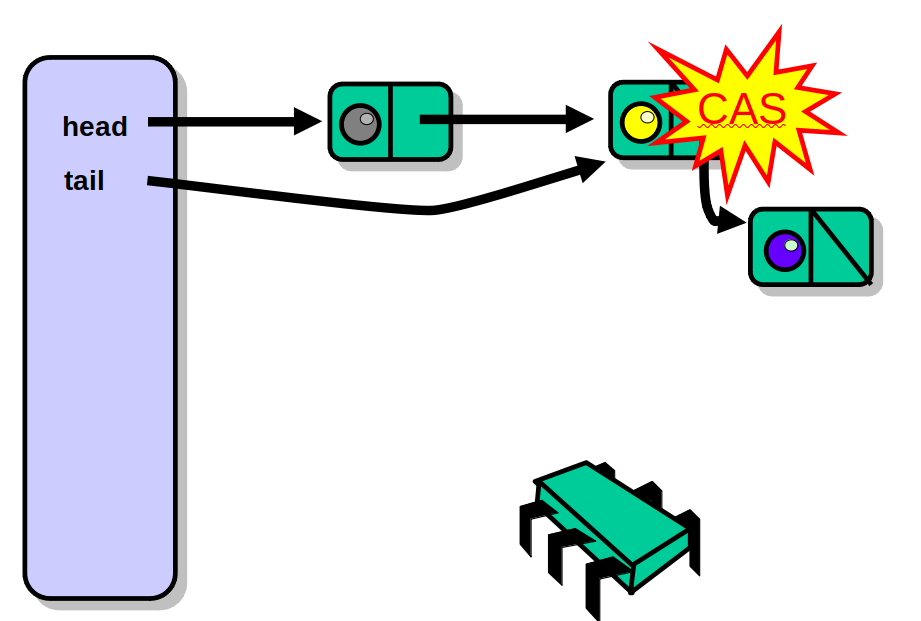
\includegraphics[width=0.7\textwidth]{./pics/unbound-mpmc/94.png} \end{center} }
\end{frame}

\begin{frame}[fragile]{Physical enqueue}
\only<1>{ \begin{center} 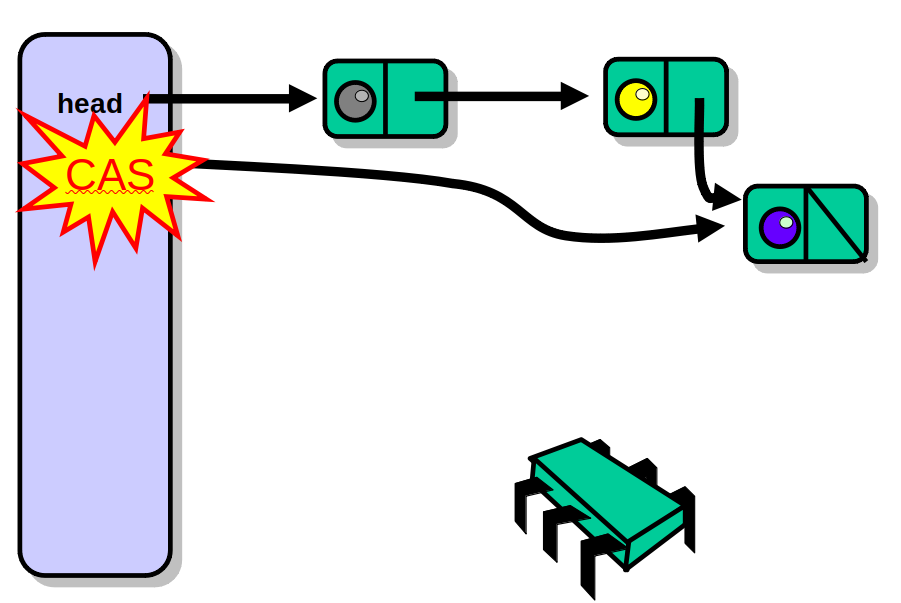
\includegraphics[width=0.7\textwidth]{./pics/unbound-mpmc/95.png} \end{center} }
\end{frame}

\begin{frame}[fragile]{Enqueue}

Logical enqueue and physical enqueue are separate steps
\begin{itemize}
  \pause \item \texttt{tail} fields refers to either
  \begin{itemize}
    \pause \item Actual last node (good)
    \pause \item "Lagging" \ node (not so good)
  \end{itemize}  
\end{itemize}

\pause 
What should we do with "trailing tail"
\begin{itemize}
  \pause \item Stop and fix it before doing anything else
  \pause \item If \texttt{tail.next != null} then CAS \texttt{tail -> tail.next}
\end{itemize}

\pause 
Why is it important
\begin{itemize}
  \pause \item Logical \texttt{enqueue}
  \begin{itemize}
    \pause \item Failed CAS means we need to restart enqueue operation
    \pause \item But still lock-free (why?)
  \end{itemize}
  \pause \item Physical \texttt{enqueue}
  \begin{itemize}
    \pause \item Failed CAS means other thread helped to fix invariants
  \end{itemize}
  \pause \item Inside \texttt{dequeue}
  \begin{itemize}
    \pause \item Actual \texttt{tail} lagging behind \texttt{head}
    \pause \item Swapping "sentinel" \ may delete actual data, make tail up-to-date before dequeue
  \end{itemize}
\end{itemize}

\end{frame}

\begin{frame}[fragile]{Dequeue}
\only<1>{ \begin{center} 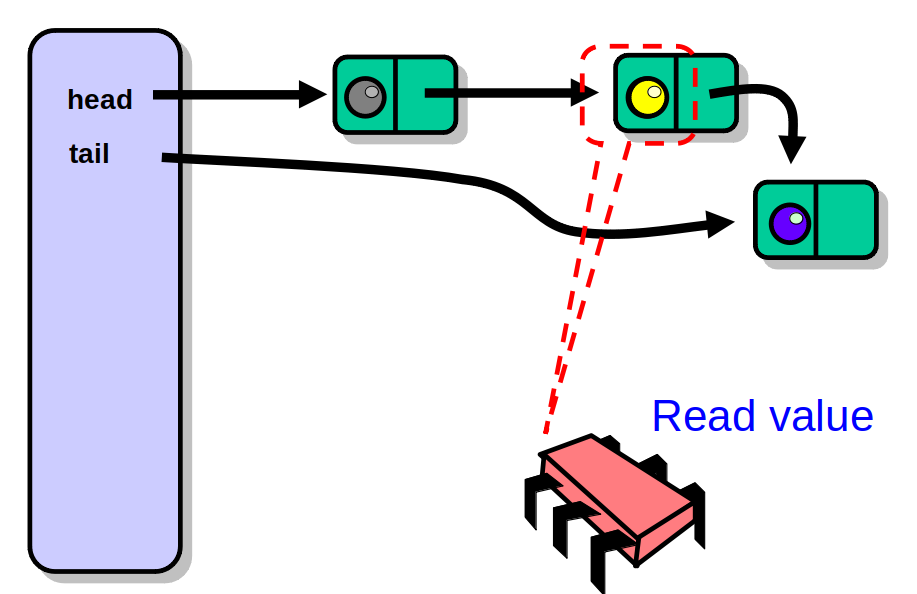
\includegraphics[width=0.7\textwidth]{./pics/unbound-mpmc/99.png} \end{center} }
\only<2>{ \begin{center} 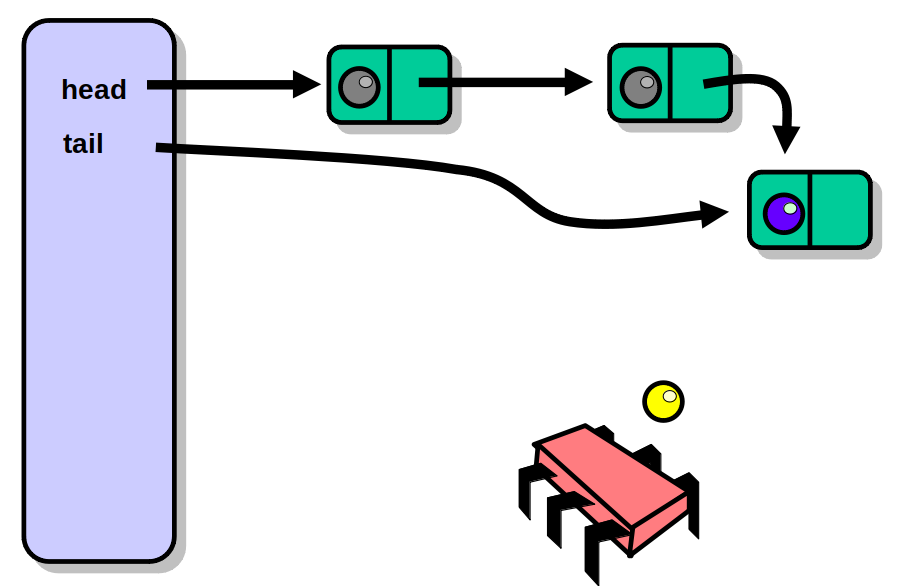
\includegraphics[width=0.7\textwidth]{./pics/unbound-mpmc/100.png} \end{center} }
\only<3>{ \begin{center} 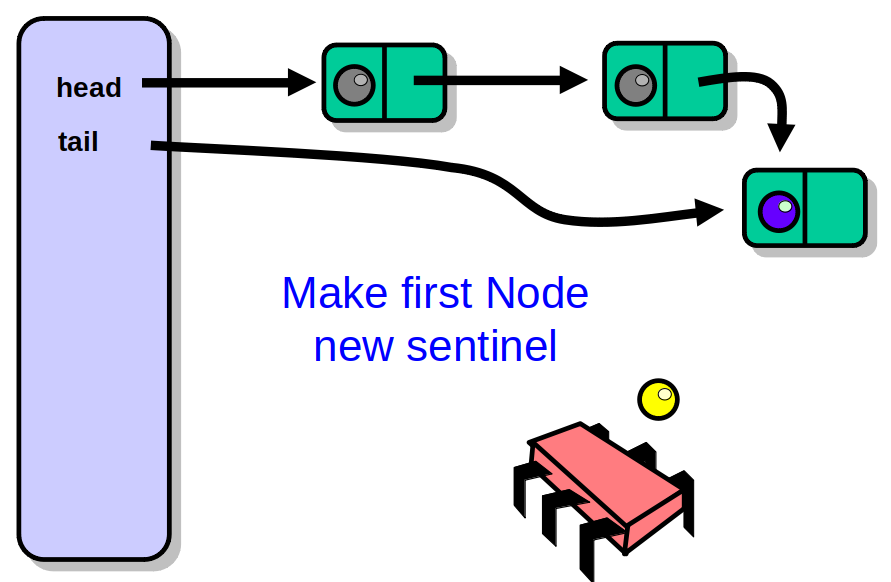
\includegraphics[width=0.7\textwidth]{./pics/unbound-mpmc/101.png} \end{center} }
\only<4>{ \begin{center} 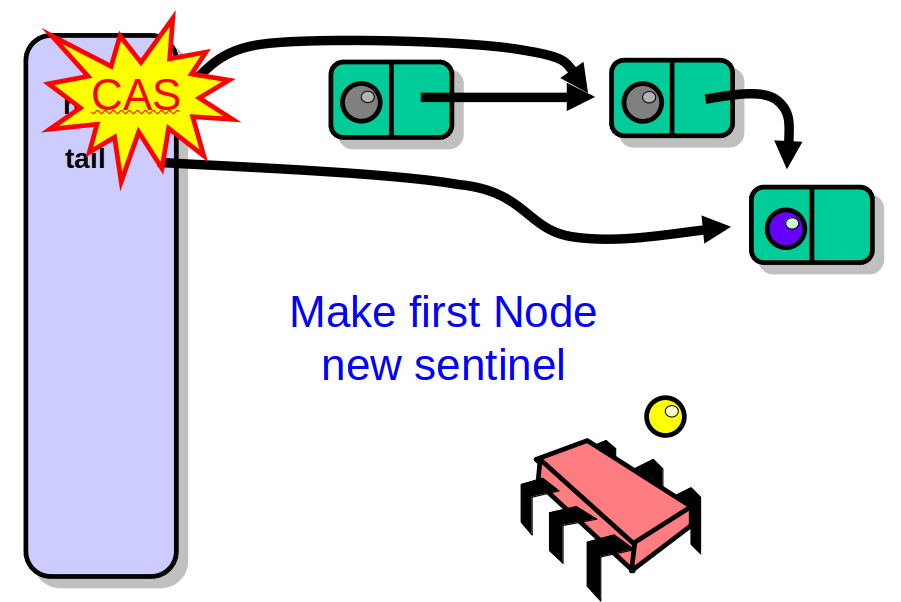
\includegraphics[width=0.7\textwidth]{./pics/unbound-mpmc/102.png} \end{center} }
\only<5>{ \begin{center} 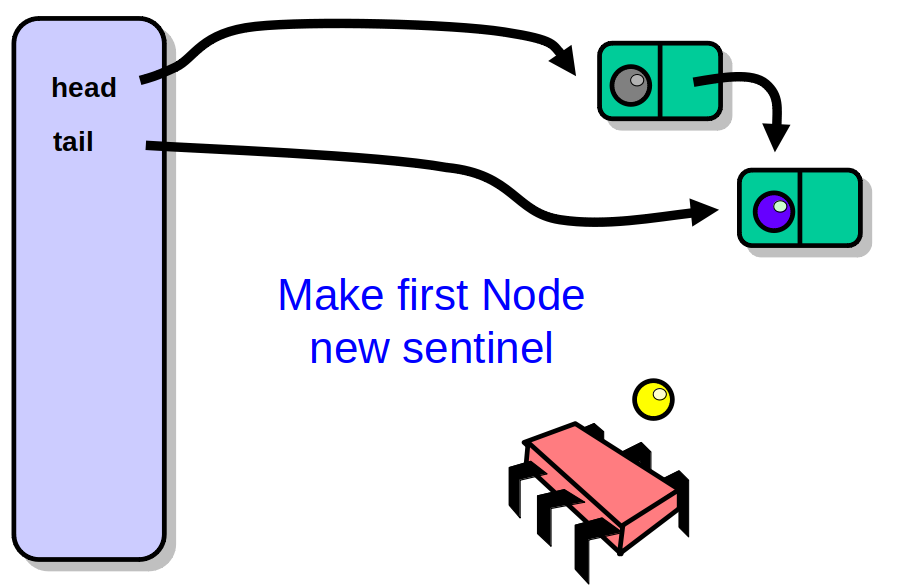
\includegraphics[width=0.7\textwidth]{./pics/unbound-mpmc/103.png} \end{center} }
\end{frame}

\begin{frame}[fragile]{Enqueue: code}

\begin{minted}{java}
public void enqueue(T value) {
  Node node = new Node(value);
  while (true) {
    Node last = tail.get();
    Node next = last.next.get();
    if (last == tail.get()) {
      if (next == null) {
        if (last.next.compareAndSet(next, node)) { // logical
          tail.compareAndSet(last, node);          // physical
          return;
        }
      } else {
        tail.compareAndSet(last, next); // repair tail and repeat
      }
}}}
\end{minted}
\end{frame}

\begin{frame}[fragile]{Dequeue: code}

\begin{minted}{java}
public T dequeue() {
  while (true) {
    Node first = head.get();
    Node last = tail.get();
    Node next = first.next.get();
    if (first == head.get()) {
      if (first == last) {
        if (next == null) throw new EmptyException();
        tail.compareAndSet(last, next); // repair tail and repeat
      } else {
        T value = next.value;
        if (head.compareAndSet(first, next)) return value;
}}}}
\end{minted}
\end{frame}

\begin{frame}{Unbounded MPMC linearizable total queue}

\begin{itemize}
  \item LinkedList-based
  \item Strong FIFO\footnote{Homework: find linearization points}
  \item Unbounded, needs Garbage Collection to avoid ABA
  \item Enqueue uses "helping hand" \ pattern to be lock-free
  \item Dequeue uses "helping hand" \ pattern to be correct
\end{itemize}

See Section 10.5 "An Unbounded Lock-Free Queue" \ in "The Art of Multiprocessor Programming" \ (pages 230 - 233).

\end{frame}


\section{Bounded array-based queues}
\showTOC

\begin{frame}{Bounded array-based queues}

\only<1>{ \begin{center} 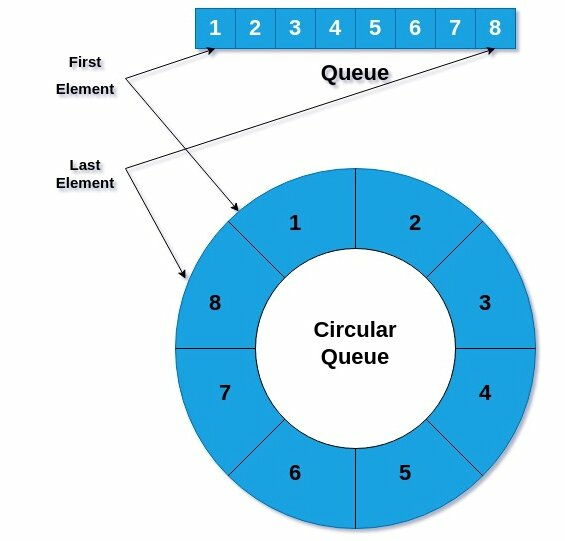
\includegraphics[width=0.4\textwidth]{./pics/circular.png} \end{center} }

\end{frame}

\subsection{SPSC}
\showTOCSub

\begin{frame}[fragile]{SPSC}

\begin{minted}{java}
class SPSC_WaitFree_Queue<T> {
  volatile int head = 0, tail = 0; T[] items = (T[]) new Object[capacity];  
  void enqueue(T x) {
    if (tail - head == items.length) throw new FullException();
    items[tail % items.length] = x;
    tail++; // not even getAndAdd
  }
  T dequeue() {
    if (tail - head == 0) throw new EmptyException();
    T x = items[head % items.length];
    head++; // not even getAndAdd
    return x;
}}
\end{minted}

\pause Could you find linearization points? Could you find memory barriers?

\end{frame}

\subsection{MPSC}
\showTOCSub

\begin{frame}{MPSC}
\end{frame}

\questiontime{How to create correct MPSC queue from \textbf{single} SPSC queue?}

\begin{frame}[t,fragile]{MPSC from N SPSC}

\begin{tikzpicture}[remember picture,overlay]
  \node[xshift=3.1cm,yshift=0.8cm] at (current page.center) {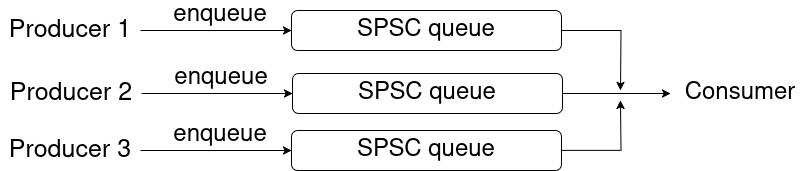
\includegraphics[width=0.6\textwidth]{./pics/mpsc.png}};
\end{tikzpicture}

\pause

\begin{minted}{java}
SPSC[] queues = ...
void enqueue(T x) {
  int id = ThreadID.get();
  queues[id].enqueue(x);
}
T dequeue() {
  for (q : queues) if (!q.isEmpty()) return q.dequeue();
  throw new EmptyException();
}
\end{minted}

\begin{itemize}
  \item Wait-free? \pause Thanks to SPSC. \pause But \texttt{dequeue} is O(T).
\end{itemize}

\end{frame}

\begin{frame}[t,fragile,noframenumbering]{MPSC from N SPSC}

\begin{tikzpicture}[remember picture,overlay]
  \node[xshift=2.7cm,yshift=-6cm] at (current page.center) {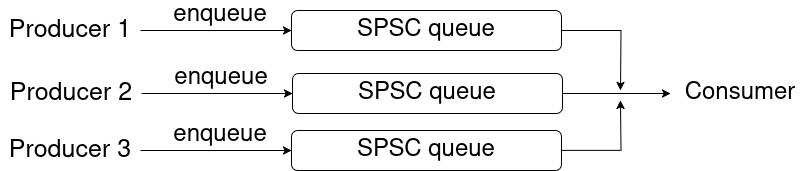
\includegraphics[width=0.6\textwidth]{./pics/mpsc.png}};
\end{tikzpicture}

\begin{minted}{java}
SPSC[] queues = ...
void enqueue(T x) {
  int id = ThreadID.get();
  queues[id].enqueue(x);
}
T dequeue() {
  for (q : queues) if (!q.isEmpty()) return q.dequeue();
  throw new EmptyException();
}
\end{minted}

\begin{itemize}  
  \item Strong FIFO?
  \begin{itemize}
    \pause \item \texttt{t1:enq(x)} $\rightarrow$ \texttt{t2:enq(y)} \textbf{does not} imply \texttt{deq(x)} $\rightarrow$ \texttt{deq(y)}
    \pause \item \texttt{t1:enq(x)} $\rightarrow$ \texttt{t1:enq(y)} \textbf{does} imply \texttt{deq(x)} $\rightarrow$ \texttt{deq(y)}    
  \end{itemize}
\end{itemize}

\end{frame}

\begin{frame}[t,fragile,noframenumbering]{MPSC from N SPSC}

\begin{tikzpicture}[remember picture,overlay]
  \node[xshift=2.7cm,yshift=-6cm] at (current page.center) {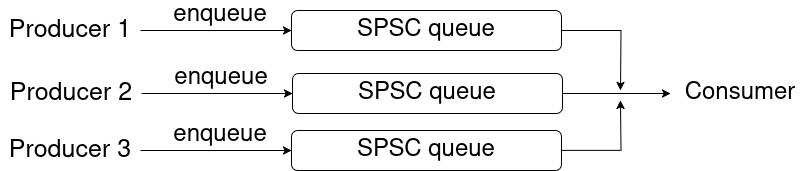
\includegraphics[width=0.6\textwidth]{./pics/mpsc.png}};
\end{tikzpicture}

\begin{minted}{java}
SPSC[] queues = ...
void enqueue(T x) {
  int id = ThreadID.get();
  queues[id].enqueue(x);
}
T dequeue() {
  for (q : queues) if (!q.isEmpty()) return q.dequeue();
  throw new EmptyException();
}
\end{minted}

\begin{itemize}  
  \item Really empty? \pause Homework: what is \textit{empty} for this queue  
\end{itemize}

\end{frame}

\begin{frame}[t,fragile]{MPSC from N SPSC}

\begin{itemize}
  \item Need to register threads in advance
  \pause \item Weak ordering guarantees
  \pause \item But wait-free!
  \pause \item \texttt{isEmpty} takes O(T)
  \pause \item Use atomic counters for \texttt{size}?
\end{itemize}
\end{frame}

\begin{frame}[t,fragile]{MPSC from N SPSC}

\begin{itemize}
  \item Use atomic counters for O(1) size check
\end{itemize}

\pause

\begin{minted}{java}
void enqueue(T x) {  
  size.getAndAdd(1);
  queues[ThreadID.get()].enqueue(x);
}
T dequeue() {
  if (size.get() == 0) throw new EmptyException();
  for (q : queues) if (!q.isEmpty()) {
    size.getAndAdd(-1);
    return q.dequeue();
  }
  assert false;
}
\end{minted}

\pause
\texttt{AssertionError}!
\end{frame}


\begin{frame}[t,fragile]{MPSC from N SPSC}

\begin{itemize}
  \item Use atomic counters for O(1) size check
\end{itemize}

\begin{minted}{java}
void enqueue(T x) {
  queues[ThreadID.get()].enqueue(x);
  size.getAndAdd(1);
}
T dequeue() {
  if (size.get() == 0) throw new EmptyException();
  for (q : queues) if (!q.isEmpty()) {
    size.getAndAdd(-1);
    return q.dequeue();
  }
  assert false;
}
\end{minted}

\pause
Missing already available element?

\end{frame}


\begin{frame}[t,fragile]{MPSC from N SPSC}

\begin{itemize}
  \item Use atomic counters for O(1) size check
\end{itemize}

\begin{minted}{java}
void enqueue(T x) {  
  queues[ThreadID.get()].enqueue(x);
  size.getAndAdd(1);
}
T dequeue() {
  while (true) {
    for (q : queues) if (!q.isEmpty()) {
      size.getAndAdd(-1); return q.dequeue();
    }
    if (size.get() == 0) throw new EmptyException();
}}
\end{minted}

\begin{itemize}
  \pause \item Wait-free?
  \pause \item Negative \texttt{size}?
\end{itemize}

\end{frame}


\begin{frame}[t,fragile]{Building queues from other queues: takeaways}

Building distributed queue from more specialized parts:
\begin{itemize}
  \pause \item \textit{Could} be scalability-friendly
  \pause \item \textit{Could} be \textit{really} non-blocking
  \pause \item \textit{Definitely will be} error-prone
  \pause \item Relaxing consistency requirements helps
  \pause \item Useful to think in terms of linearization points
  \begin{itemize}
    \pause \item Operation takes effect \textbf{here}
    \pause \item Even if the whole API is not linearizable
  \end{itemize}
\end{itemize}

\pause

Specialized lock-free single-queue algorithms exist: 
\begin{itemize}
  \item JCTools 
  \begin{itemize}
    \item \url{https://github.com/JCTools/JCTools}
    \item \url{https://www.infoq.com/presentations/jctools-algorithms-optimization}
  \end{itemize}
  \item 1024 cores
  \begin{itemize}
    \item \url{https://www.1024cores.net/home/lock-free-algorithms/queues}  
  \end{itemize}
\end{itemize}
\end{frame}

\subsection{SPMC}
\showTOCSub

\begin{frame}[fragile]{SPMC}
\end{frame}

\questiontime{How to build SPMC queue from \textbf{one} single-producer \textbg{k}-consumer queue?}

\begin{frame}[t,fragile]{SPMC from N SPSC}

\begin{tikzpicture}[remember picture,overlay]
  \node[xshift=2.7cm,yshift=-7cm] at (current page.center) {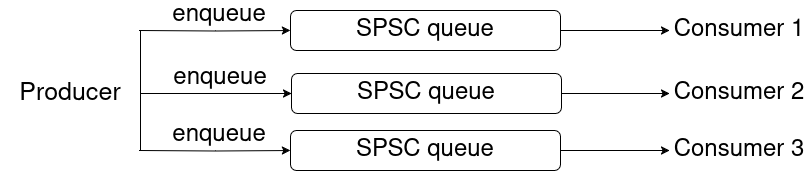
\includegraphics[width=0.6\textwidth]{./pics/spmc.png}};
\end{tikzpicture}

\pause

\begin{minted}{java}
SPSC[] queues = ...
void enqueue(T x) {
  for (q : queues) if (!q.isFull()) {
    q.enqueue(x); return;
  }
  throw new FullException();
}
T dequeue() {  
  return queues[ThreadID.get()].dequeue();  
}
\end{minted}

\pause
\begin{itemize}
  \item What is empty queue?
  \begin{itemize}
    \pause \item Producer view: all consumer queues are empty
    \pause \item Consumer view: my queue is empty
  \end{itemize}
\end{itemize}
\end{frame}

\begin{frame}[t,fragile,noframenumbering]{SPMC from N SPSC}

\begin{tikzpicture}[remember picture,overlay]
  \node[xshift=2.7cm,yshift=-7cm] at (current page.center) {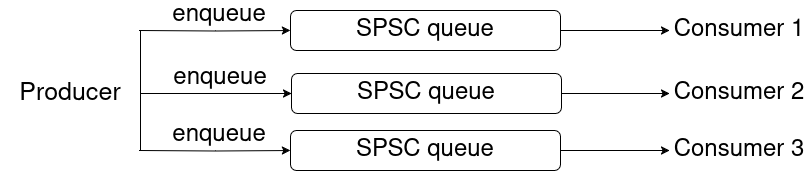
\includegraphics[width=0.6\textwidth]{./pics/spmc.png}};
\end{tikzpicture}

\begin{minted}{java}
SPSC[] queues = ...
void enqueue(T x) {
  for (q : queues) if (!q.isFull()) {
    q.enqueue(x); return;
  }
  throw new FullException();
}
T dequeue() {  
  return queues[ThreadID.get()].dequeue();  
}
\end{minted}

\begin{itemize}
  \item Linearizability? \pause No, but maybe OK
  \pause \item Load balancing? \pause No, definitely not OK      
\end{itemize}
\end{frame}

\begin{frame}[t,fragile,noframenumbering]{SPMC from N SPSC}

\begin{itemize}
  \item Naive work-stealing as load balancing strategy
\end{itemize}

\pause

\begin{minted}{java}
void enqueue(T x) {
  for (q : queues) synchronized(q) { if (!q.isFull()) {
    q.enqueue(x); return;
  }}
  throw new FullException();
}
T dequeue() {  
  SPSC q = queues[ThreadID.get()];
  synchronized(q) { if (!q.isEmpty()) return q.dequeue(); }  
  for(q : queues) synchronized(q) { if (!q.isEmpty()) return q.dequeue(x); }
}
\end{minted}

\pause
\begin{itemize}
  \item Real-life algorithms: batch steal, lock-free steal
\end{itemize}

\end{frame}


\begin{frame}[t,fragile]{Consumer contention: takeaways}

\begin{itemize}
  \item Many producers/consumers -- maybe strong FIFO is not that necessary
  \pause \item Many consumers -- load balancing required
  \pause \item Non-blocking work stealing looks like hard problem
\end{itemize}

\pause

Specialized lock-free single-queue algorithms exist: 
\begin{itemize}
  \item JCTools 
  \begin{itemize}
    \item \url{https://github.com/JCTools/JCTools}
    \item \url{https://www.infoq.com/presentations/jctools-algorithms-optimization}
  \end{itemize}
  \item 1024 cores
  \begin{itemize}
    \item \url{https://www.1024cores.net/home/lock-free-algorithms/queues}  
  \end{itemize}
\end{itemize}

\end{frame}


\section{Concurrent DEQueue and work stealing}
\showTOC

\begin{frame}{Lock-Free Work Stealing}

\begin{itemize}
  \pause \item Each thread has a pool of ready work
  \pause \item Remove work without synchronizing
  \pause \item If you run out of work, steal from someone
  \pause \item Choose victim at random
\end{itemize}

\end{frame}

\begin{frame}{Local work pools}
\only<1>{ \begin{center} 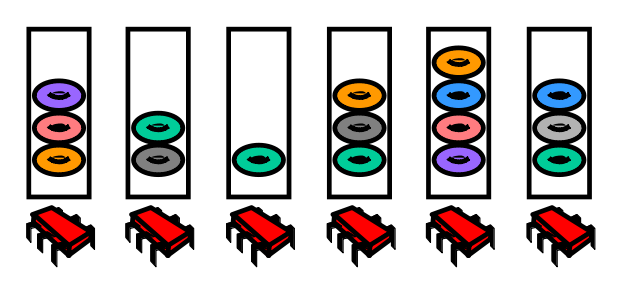
\includegraphics[width=0.6\textwidth]{./pics/work-steal/91.png} \end{center} }
\end{frame}

\begin{frame}[noframenumbering]{DoubleEndedQueue}
\only<1>{ \begin{center} 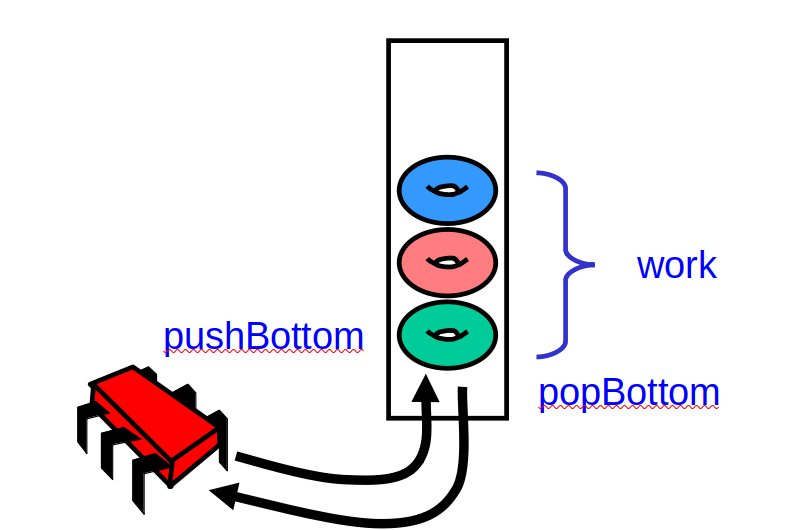
\includegraphics[width=0.6\textwidth]{./pics/work-steal/92.png} \end{center} }
\end{frame}

\begin{frame}[noframenumbering]{Obtain work}
\only<1>{ \begin{center} 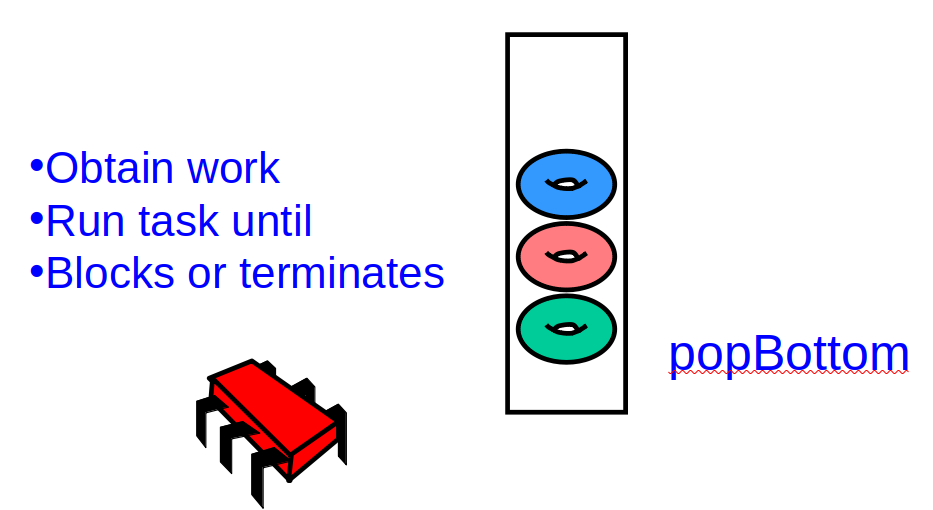
\includegraphics[width=0.6\textwidth]{./pics/work-steal/93.png} \end{center} }
\end{frame}

\begin{frame}[noframenumbering]{New work}
\only<1>{ \begin{center} 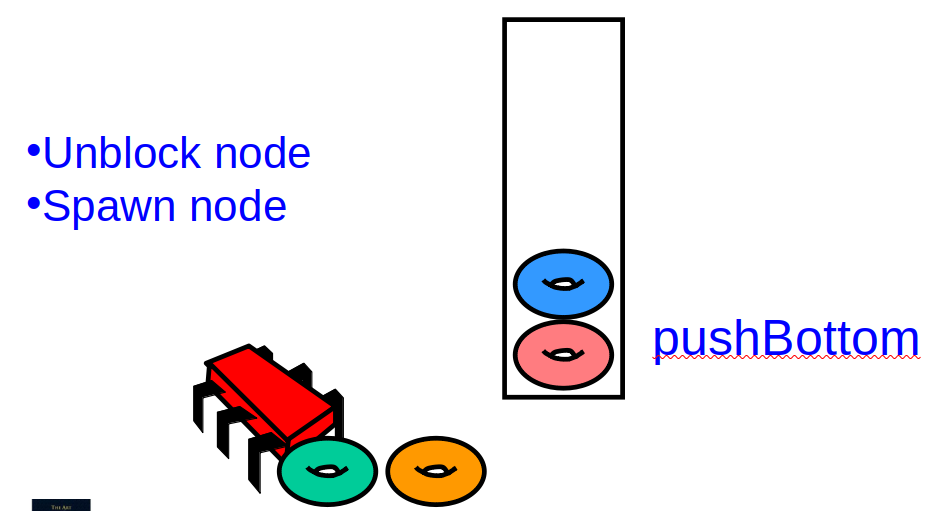
\includegraphics[width=0.6\textwidth]{./pics/work-steal/94.png} \end{center} }
\end{frame}

\begin{frame}[noframenumbering]{Out of work}
\only<1>{ \begin{center} 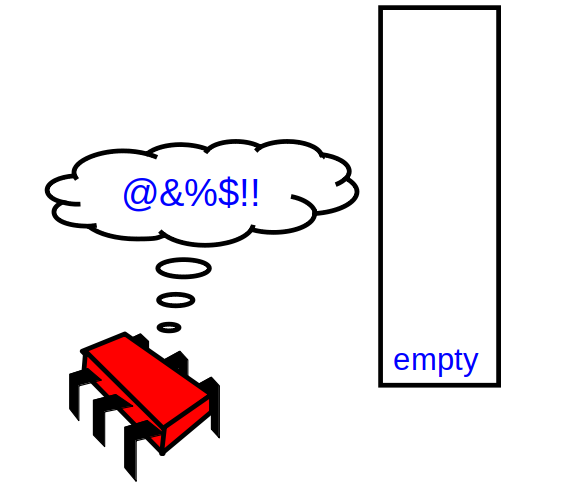
\includegraphics[width=0.5\textwidth]{./pics/work-steal/95.png} \end{center} }
\end{frame}

\begin{frame}[noframenumbering]{Steal from others}
\only<1>{ \begin{center} 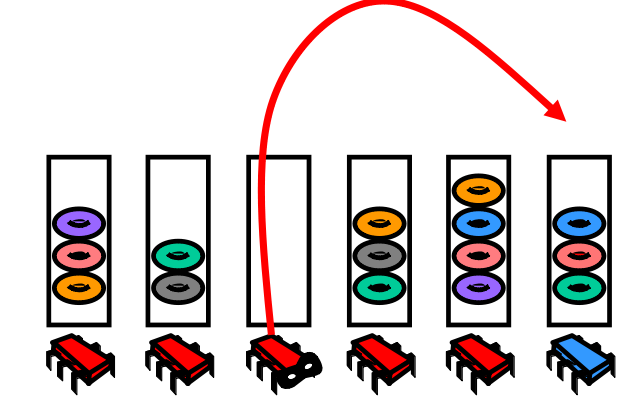
\includegraphics[width=0.6\textwidth]{./pics/work-steal/96.png} \end{center} }
\end{frame}

\begin{frame}[noframenumbering]{Steal task}
\only<1>{ \begin{center} 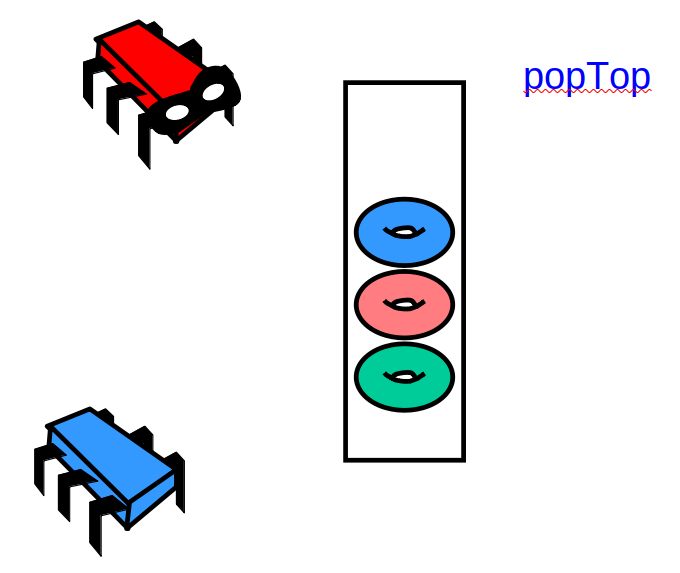
\includegraphics[width=0.5\textwidth]{./pics/work-steal/97.png} \end{center} }
\end{frame}

\begin{frame}{Task DEQueue}

Methods:
\begin{itemize}
  \item \texttt{pushBottom}, \texttt{popBottom}, \texttt{popTop}
\end{itemize}

\pause
\texttt{pushBottom} and \texttt{popBottom} are never concurrent:
\begin{itemize}
  \pause \item make them fast
  \pause \item minimize use of CAS
\end{itemize}

\pause
Ideal requirements:
\begin{itemize}
  \item Wait-Free, Linearizable, Constant time
\end{itemize}

\pause

Compromise: \pause method \texttt{popTop} may fail if \pause
\begin{itemize}
  \item Concurrent \texttt{popTop} succeeds or 
  \item Concurrent \texttt{popBottom} takes last task  
\end{itemize}

\end{frame}

\begin{frame}{ABA problem}
\only<1>{ \begin{center} 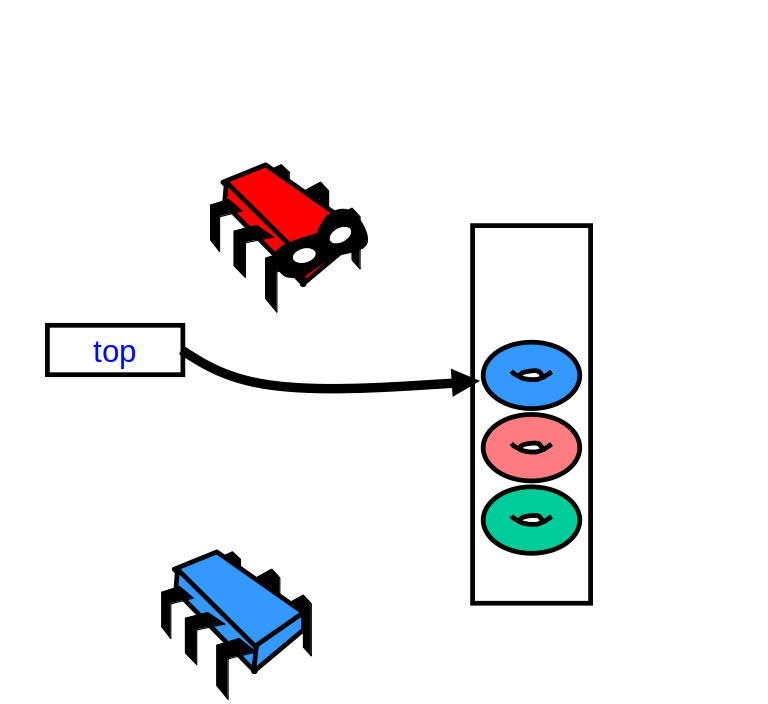
\includegraphics[width=0.4\textwidth]{./pics/work-steal/102.png} \end{center} }
\only<2>{ \begin{center} 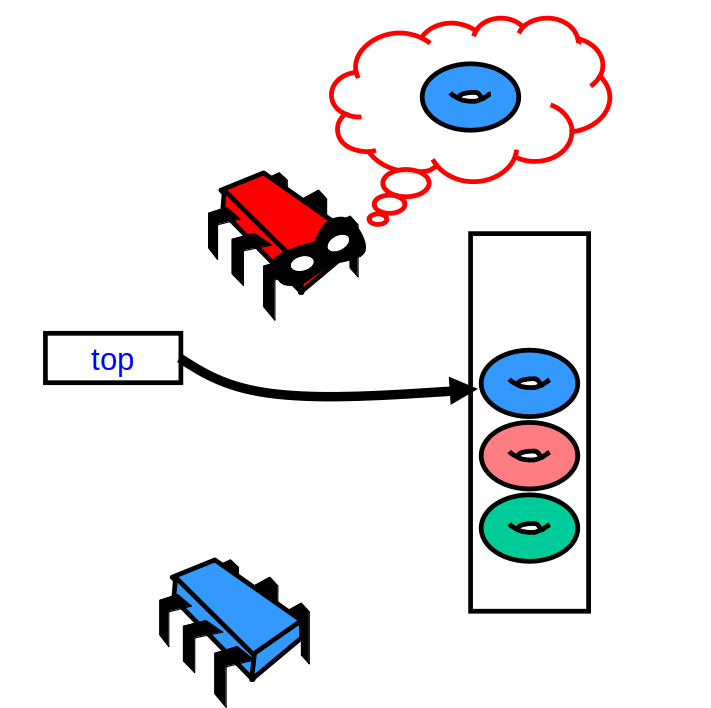
\includegraphics[width=0.4\textwidth]{./pics/work-steal/103.png} \end{center} }
\only<3>{ \begin{center} 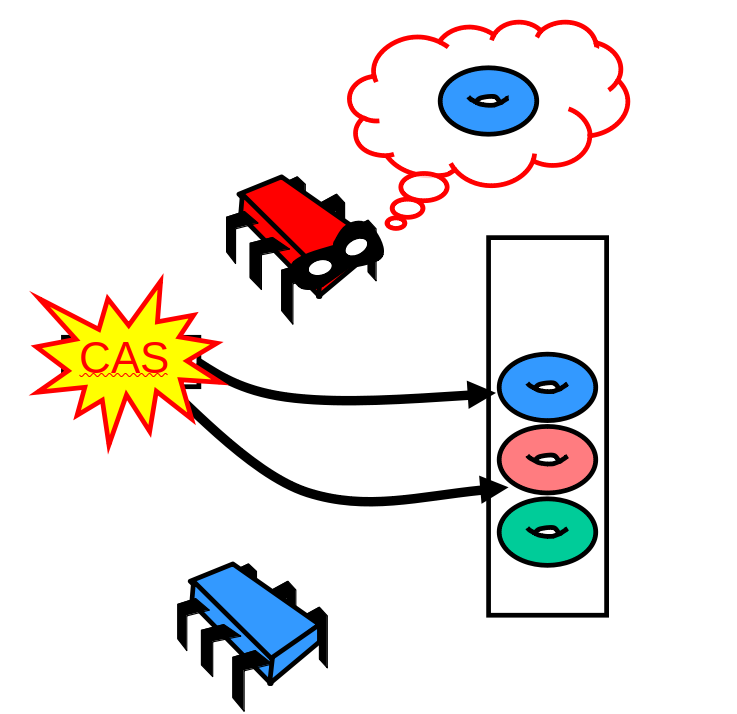
\includegraphics[width=0.4\textwidth]{./pics/work-steal/104.png} \end{center} }
\only<4>{ \begin{center} 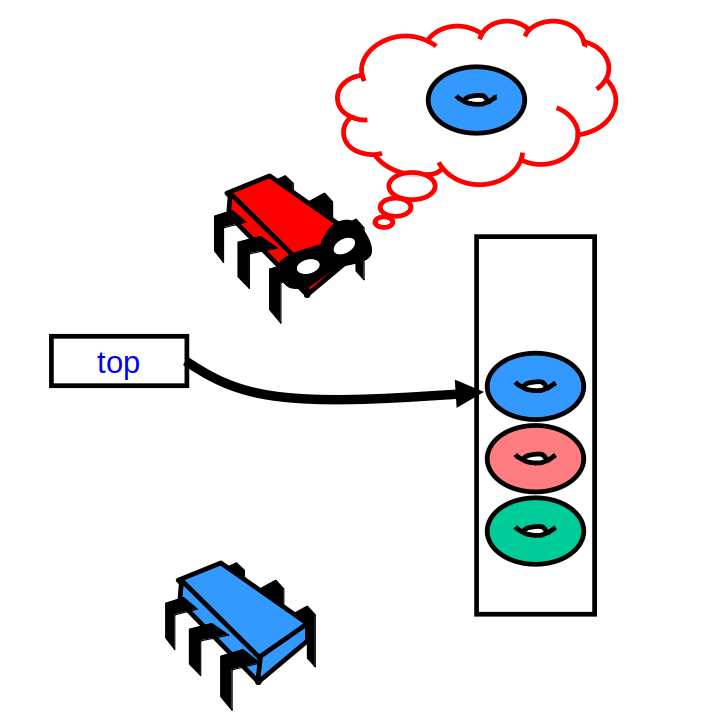
\includegraphics[width=0.4\textwidth]{./pics/work-steal/105.png} \end{center} }
\only<5>{ \begin{center} 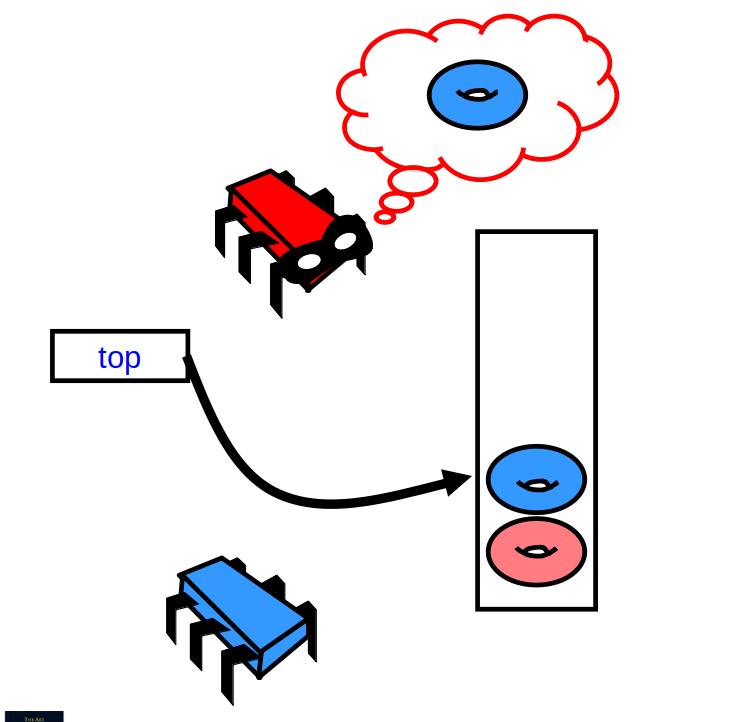
\includegraphics[width=0.4\textwidth]{./pics/work-steal/106.png} \end{center} }
\only<6>{ \begin{center} 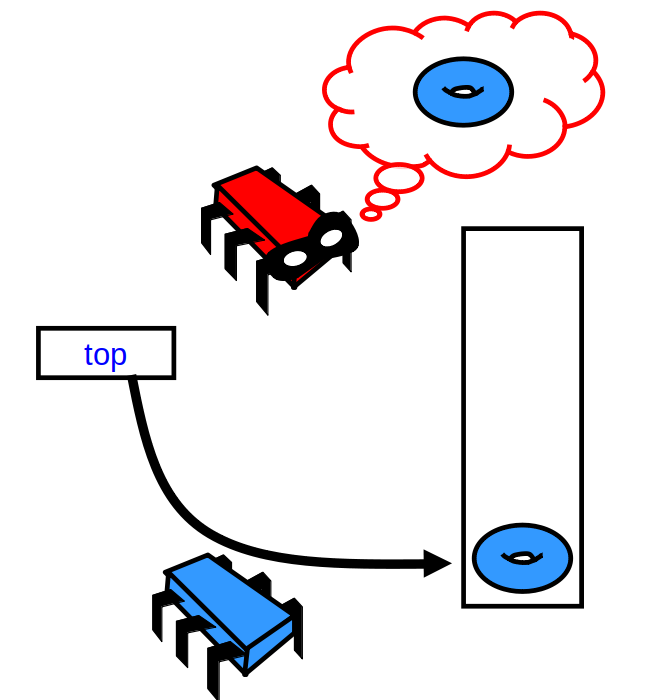
\includegraphics[width=0.4\textwidth]{./pics/work-steal/107.png} \end{center} }
\only<7>{ \begin{center} 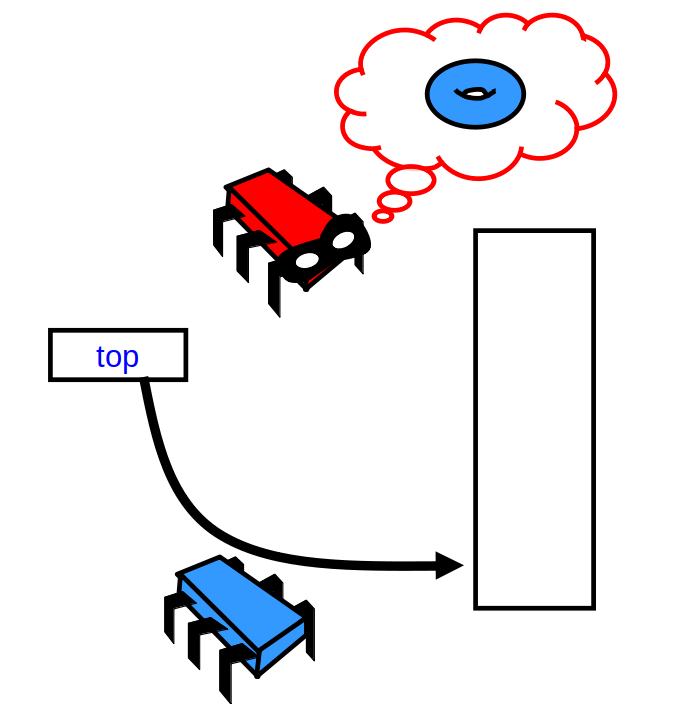
\includegraphics[width=0.4\textwidth]{./pics/work-steal/108.png} \end{center} }
\only<8>{ \begin{center} 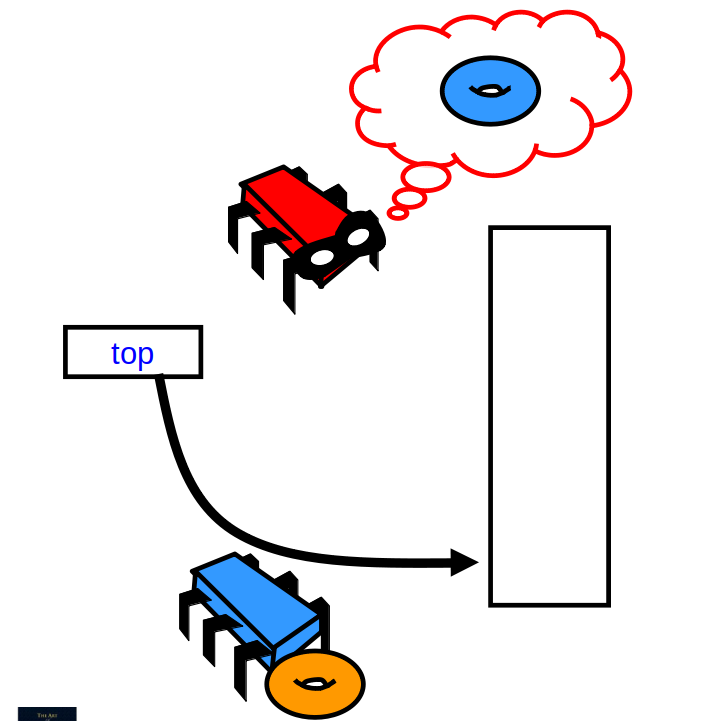
\includegraphics[width=0.4\textwidth]{./pics/work-steal/109.png} \end{center} }
\only<9>{ \begin{center} 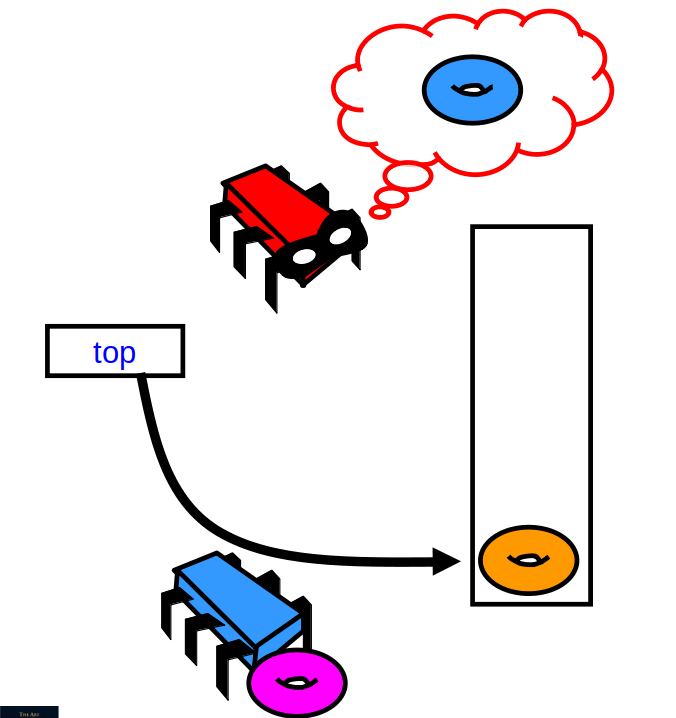
\includegraphics[width=0.4\textwidth]{./pics/work-steal/110.png} \end{center} }
\only<10>{ \begin{center} 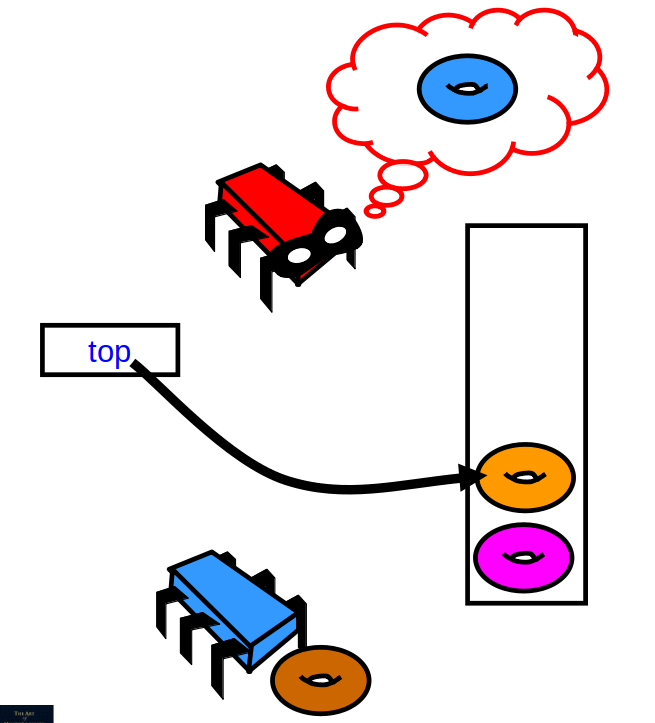
\includegraphics[width=0.4\textwidth]{./pics/work-steal/111.png} \end{center} }
\only<11>{ \begin{center} 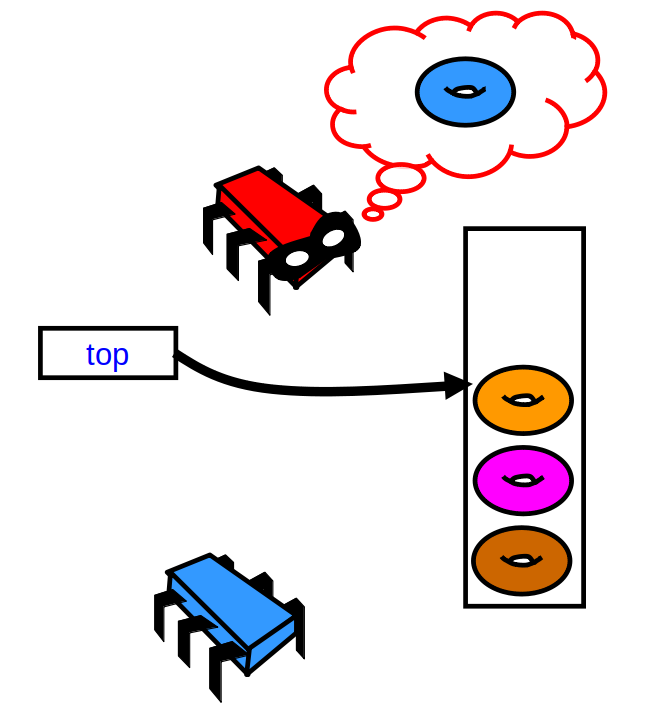
\includegraphics[width=0.4\textwidth]{./pics/work-steal/112.png} \end{center} }
\only<12>{ \begin{center} 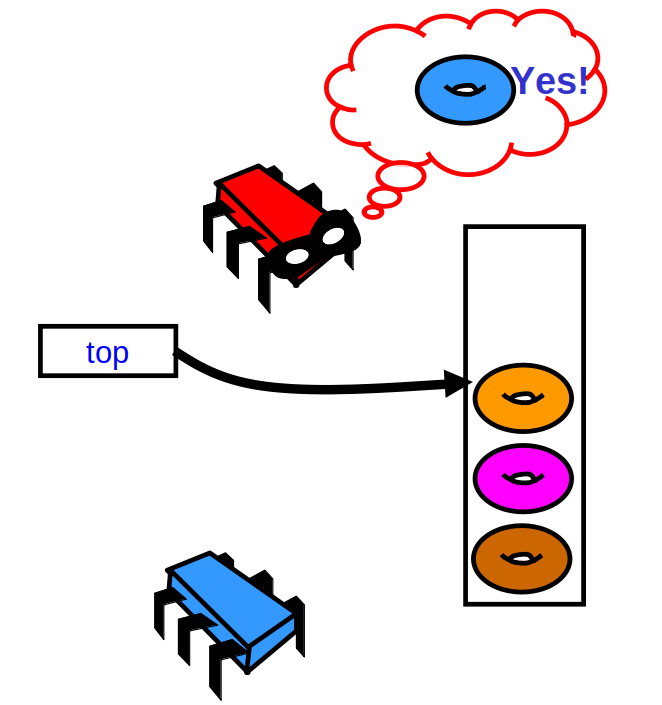
\includegraphics[width=0.4\textwidth]{./pics/work-steal/113.png} \end{center} }
\only<13>{ \begin{center} 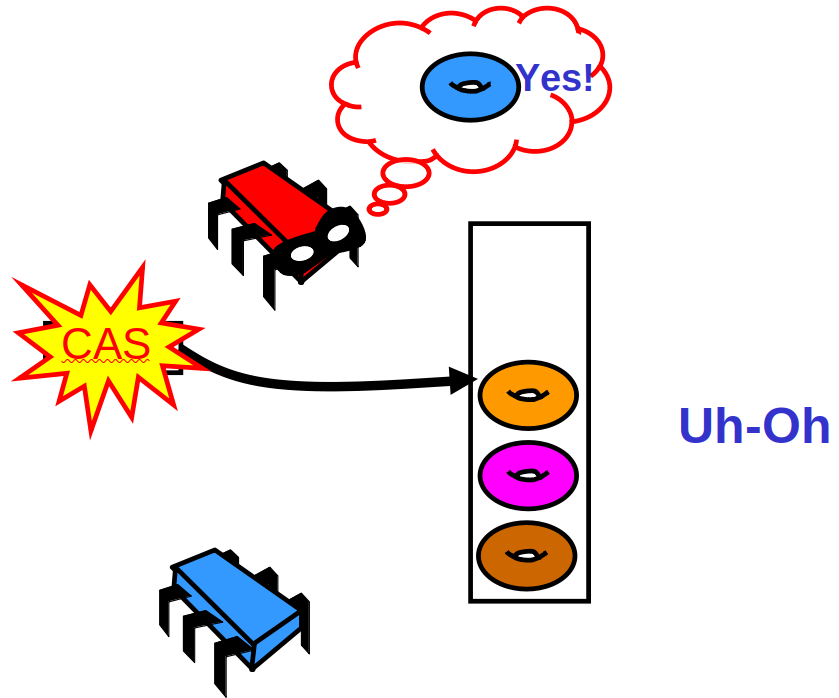
\includegraphics[width=0.5\textwidth]{./pics/work-steal/114.png} \end{center} }

\end{frame}

\begin{frame}{Fix for ABA problem}
\only<1>{ \begin{center} 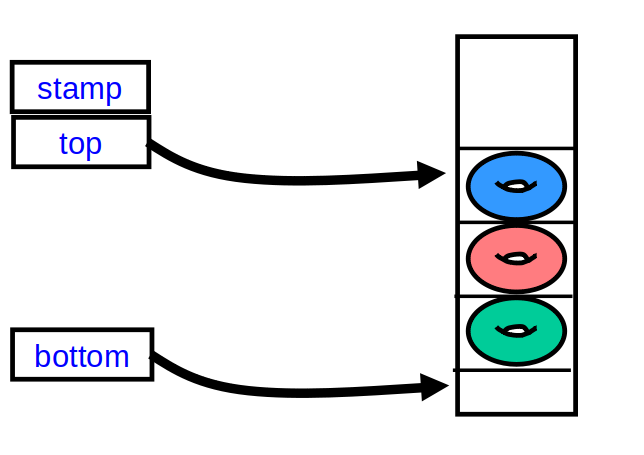
\includegraphics[width=0.4\textwidth]{./pics/work-steal/115.png} \end{center} }
\end{frame}

\begin{frame}{Bounded DEQueue}

\only<1>{ \begin{center} 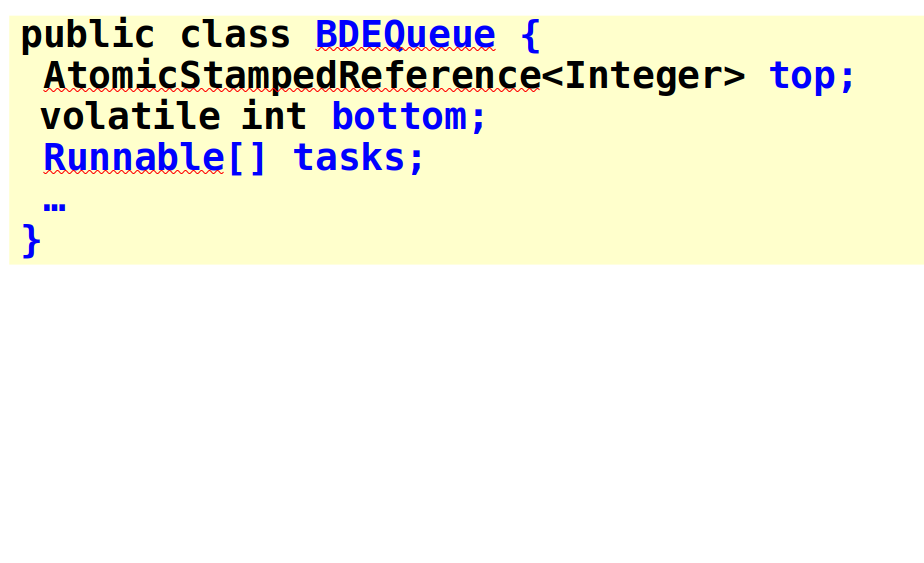
\includegraphics[width=0.6\textwidth]{./pics/work-steal/116.png} \end{center} }
\only<2>{ \begin{center} 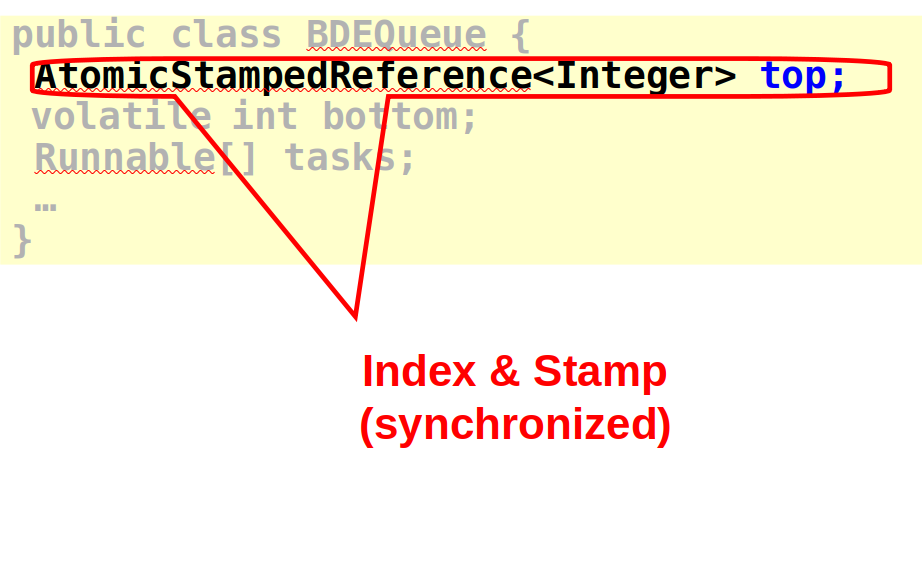
\includegraphics[width=0.6\textwidth]{./pics/work-steal/117.png} \end{center} }
\only<3>{ \begin{center} 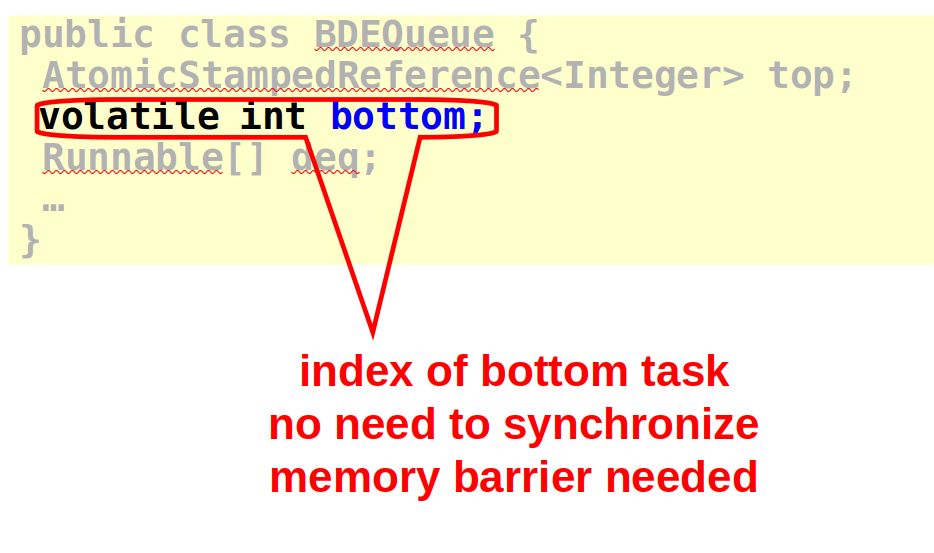
\includegraphics[width=0.6\textwidth]{./pics/work-steal/118.png} \end{center} }
\only<4>{ \begin{center} 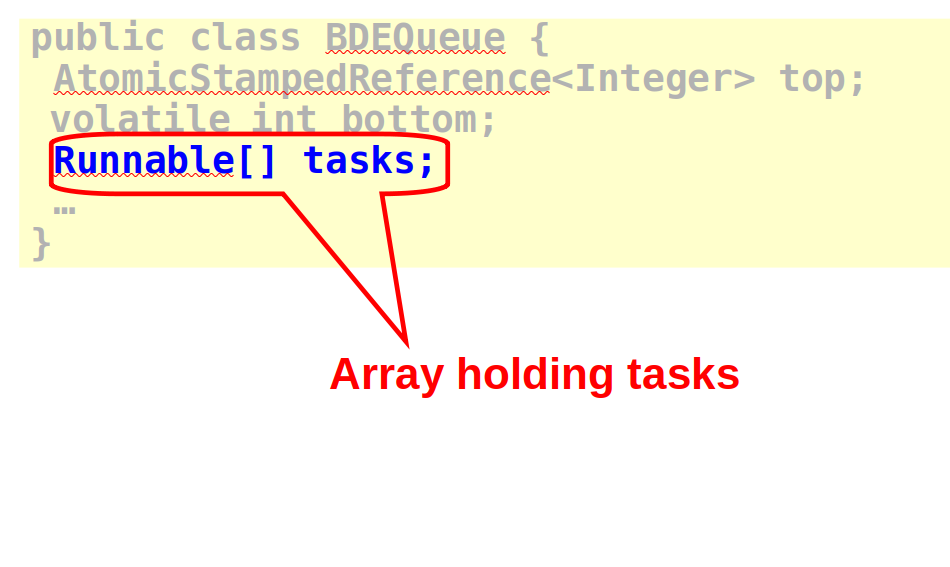
\includegraphics[width=0.6\textwidth]{./pics/work-steal/119.png} \end{center} }

\end{frame}

\begin{frame}{pushBottom}

\only<1>{ \begin{center} 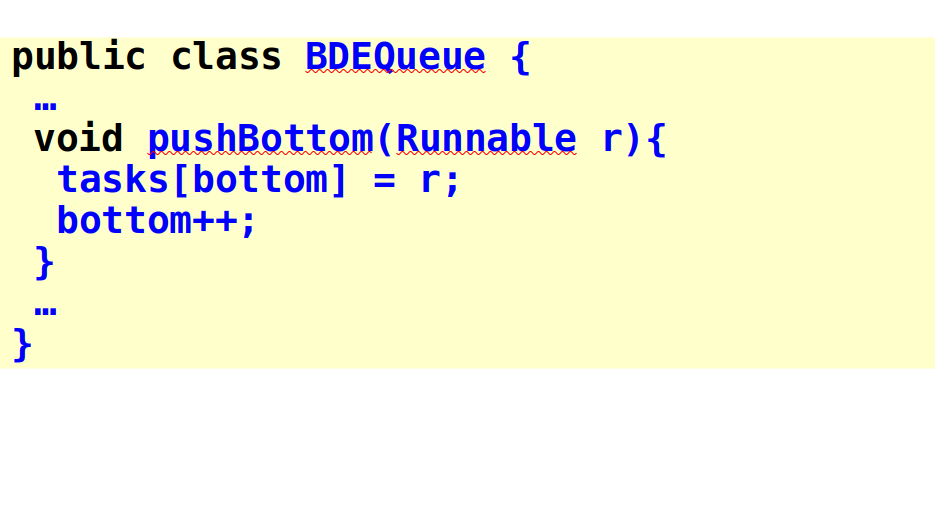
\includegraphics[width=0.6\textwidth]{./pics/work-steal/120.png} \end{center} }
\only<2>{ \begin{center} 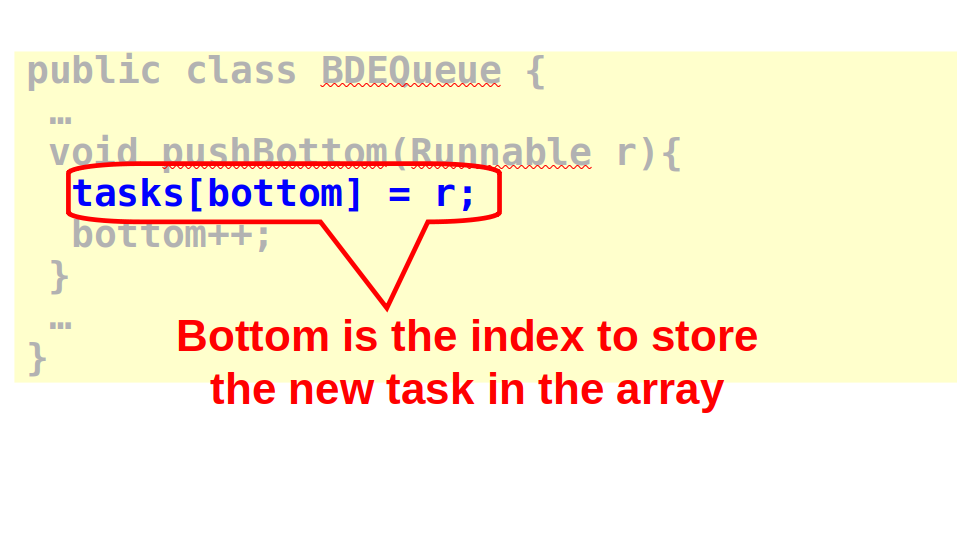
\includegraphics[width=0.6\textwidth]{./pics/work-steal/121.png} \end{center} }
\only<3>{ \begin{center} 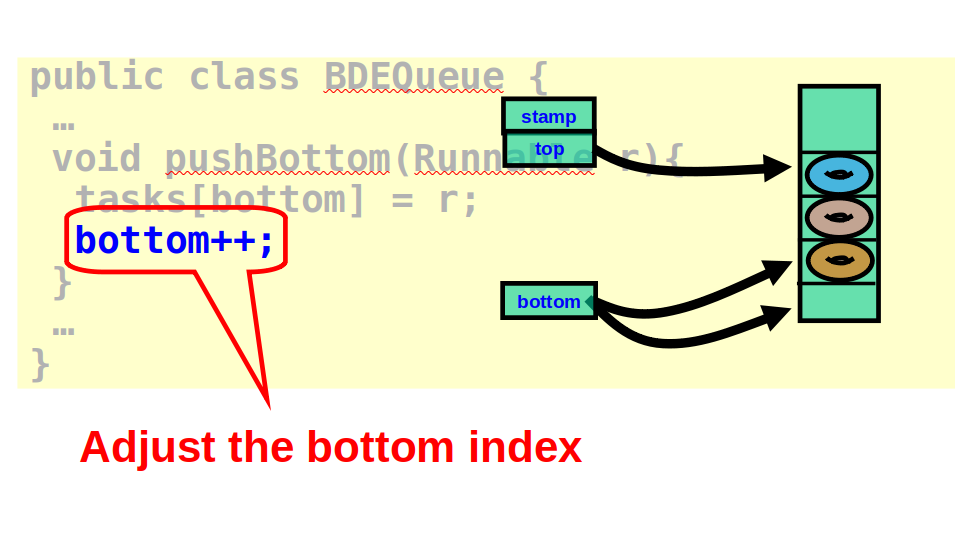
\includegraphics[width=0.6\textwidth]{./pics/work-steal/122.png} \end{center} }

\end{frame}

\begin{frame}{Steal work}

\only<1>{ \begin{center} 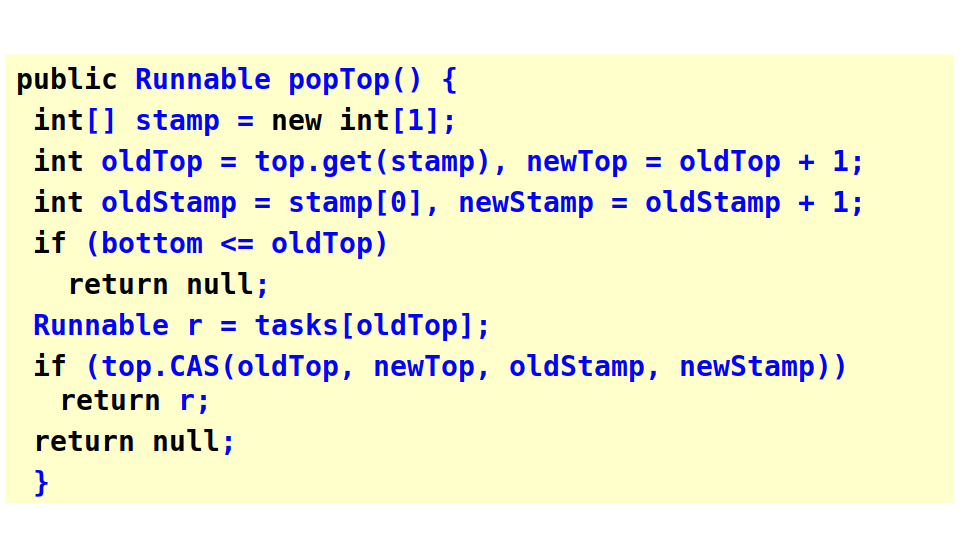
\includegraphics[width=0.6\textwidth]{./pics/work-steal/123.png} \end{center} }
\only<2>{ \begin{center} 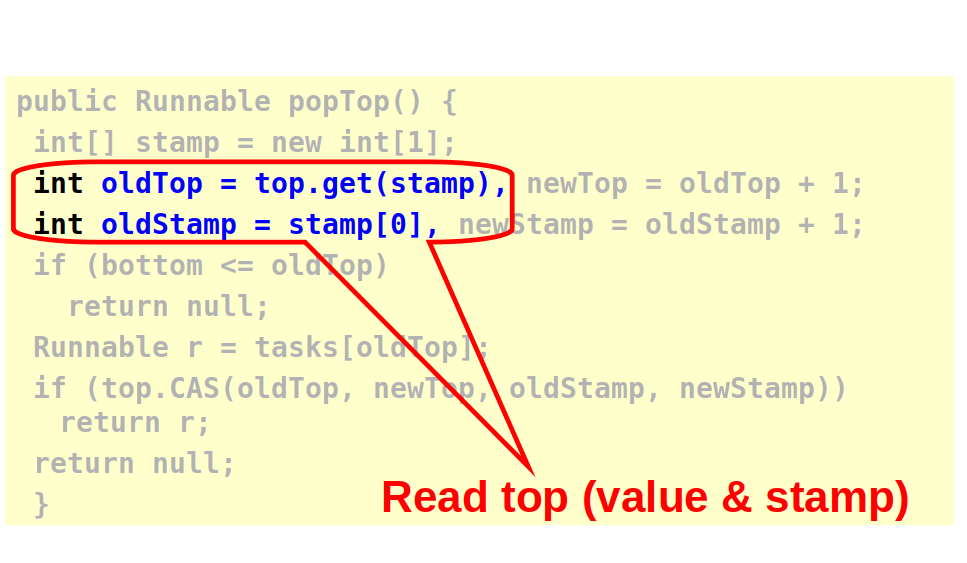
\includegraphics[width=0.6\textwidth]{./pics/work-steal/124.png} \end{center} }
\only<3>{ \begin{center} 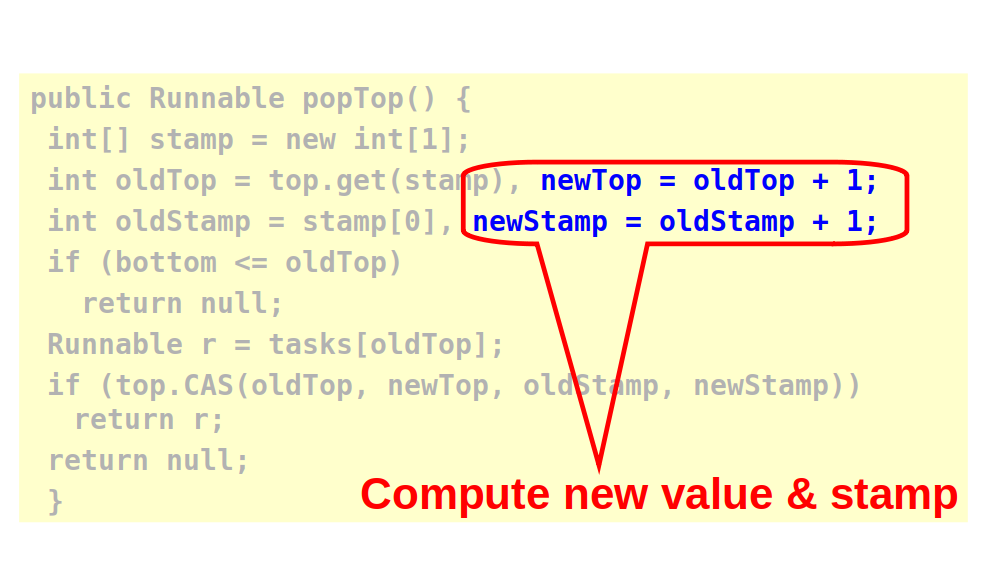
\includegraphics[width=0.6\textwidth]{./pics/work-steal/125.png} \end{center} }
\only<4>{ \begin{center} \includegraphics[width=0.6\textwidth]{./pics/work-steal/126.png} \end{center} }
\only<5>{ \begin{center} \includegraphics[width=0.6\textwidth]{./pics/work-steal/127.png} \end{center} }
\only<6>{ \begin{center} \includegraphics[width=0.6\textwidth]{./pics/work-steal/128.png} \end{center} }
\only<7>{ \begin{center} \includegraphics[width=0.6\textwidth]{./pics/work-steal/129.png} \end{center} }
\only<8>{ \begin{center} \includegraphics[width=0.6\textwidth]{./pics/work-steal/130.png} \end{center} }

\end{frame}


\begin{frame}{Take work}

\only<1>{ \begin{center} \includegraphics[width=0.6\textwidth]{./pics/work-steal/131.png} \end{center} }
\only<2>{ \begin{center} \includegraphics[width=0.6\textwidth]{./pics/work-steal/132.png} \end{center} }
\only<3>{ \begin{center} \includegraphics[width=0.6\textwidth]{./pics/work-steal/133.png} \end{center} }
\only<4>{ \begin{center} \includegraphics[width=0.6\textwidth]{./pics/work-steal/134.png} \end{center} }
\only<5>{ \begin{center} \includegraphics[width=0.6\textwidth]{./pics/work-steal/135.png} \end{center} }
\only<6>{ \begin{center} \includegraphics[width=0.6\textwidth]{./pics/work-steal/136.png} \end{center} }
\only<7>{ \begin{center} \includegraphics[width=0.6\textwidth]{./pics/work-steal/137.png} \end{center} }
\only<8>{ \begin{center} \includegraphics[width=0.6\textwidth]{./pics/work-steal/138.png} \end{center} }
\only<9>{ \begin{center} \includegraphics[width=0.6\textwidth]{./pics/work-steal/139.png} \end{center} }

\only<10>{ \begin{center} \includegraphics[width=0.6\textwidth]{./pics/work-steal/140.png} \end{center} }
\only<11>{ \begin{center} \includegraphics[width=0.6\textwidth]{./pics/work-steal/141.png} \end{center} }
\only<12>{ \begin{center} \includegraphics[width=0.6\textwidth]{./pics/work-steal/142.png} \end{center} }
\only<13>{ \begin{center} \includegraphics[width=0.6\textwidth]{./pics/work-steal/143.png} \end{center} }
\only<14>{ \begin{center} \includegraphics[width=0.6\textwidth]{./pics/work-steal/144.png} \end{center} }
\only<15>{ \begin{center} \includegraphics[width=0.6\textwidth]{./pics/work-steal/145.png} \end{center} }
\only<16>{ \begin{center} \includegraphics[width=0.6\textwidth]{./pics/work-steal/146.png} \end{center} }

\end{frame}


\begin{frame}{Work stealing and balancing}

\begin{itemize}
  \item Trade-offs: fast-path/slow-path, FIFO/LIFO, lock-free/obstruction-free, steal size
  \pause \item Clean separation between app and scheduling layer
  \pause \item Works well when number of processors fluctuates
  \pause \item Works on "black-box" \ operating systems
\end{itemize}

\end{frame}

\section{Summary}

\begin{frame}{Summary}

Queues are quite universal construct:
\begin{itemize}
  \item Concurrency control (mutex, latch, semaphore)
  \item Data transfer
  \item Load balancing
\end{itemize}

Design space:
\begin{itemize}
  \item Strong FIFO, per-producer FIFO, best-effort FIFO
  \item SPSC, MPSC, SPMC, MPMC  
  \item Bounded, unbounded
  \item Total, partial, synchronous methods
  \item Wait-free/lock-free/blocking enqueuers/dequeuers
\end{itemize}

Load balancing using DoubleEndedQueue
\begin{itemize}
  \item bottom-oriented LIFO for local tasks
  \item top-oriented work-stealing
\end{itemize}

\end{frame}

\end{document}


